\documentclass[a4paper,11pt, notitlepage]{report}
\usepackage[T1]{fontenc}
\usepackage[utf8]{inputenc}
\usepackage{lmodern}
\usepackage{graphicx}
\usepackage{listings}
\usepackage{amsmath}
\usepackage{amssymb}
\usepackage{multirow}
\usepackage{sectsty}
\usepackage{titlesec}
\usepackage{lipsum}
\usepackage{amsthm}
\usepackage{subcaption}
\usepackage{multirow}
\usepackage{titling}
\usepackage{blindtext}

\theoremstyle{definition}
\newtheorem{definition}{Definition}[section]
\newtheorem{theorem}{Theorem}[section]
\newtheorem{corollary}{Corollary}[section]
\newtheorem{lemma}{Lemma}[section]
\newtheorem{proposition}{Proposition}[section]

\chaptertitlefont{\fontsize{20pt}{15pt}\selectfont}

\title{Toposic structure theory of computations}
\author{John Bernier}

\begin{document}

\maketitle
\begin{abstract}
The theory of data-flow analysis of computer programs has been extensively studied. The increasing need for dataflow analysis in the automatic parallelization of computer programs motivates the development of mathematical foundations for this field. We present a new approach to program dataflow analysis that incorporates partition lattices and the Sierpinski topos.
\end{abstract}

\tableofcontents

\chapter{Introduction}
Richard Dedekind and Georg Cantor developed set theory in the 1870s before the first inklings of computer technology had been developed. Set theory has as its basic objects sets. This stands in contrast to most branches of mathematics, including those related to computer science, for which the fundamental objects are functions.

In computer science, functions tend to be a better core primitive of study then sets. Hence the influx of functional programming languages into the computing industry. Similarly, sets are often better treated as special cases of boolean-valued functions than primitive objects in their own right. This suggests that the Sierpinski topos $Sets^{\to}$, which takes functions rather than sets as its basic objects, is a better foundation for most applications than set theory.

A second issue with the traditional set-theoretic approach is its overreliance on subobjects to the detriment of the categorical dual logic of quotients. Several authors, including David Ellerman and Giancarlo Rota, have emphasized the dual role that partitions play to subsets in category theory, arising from the duality between monomorphisms and epimorphisms. [1] [2]

We combine these two ideas to consider the categorically dual logic of quotients in $Sets^{\to}$. The resulting construct can be used to define dataflow relations for any function that describe how functions map information from one location in a structure to another. Combined with our understanding of information locality using set partitions, this leads to our theory of local computation.

In order to study this categorically dual logic of quotients in $Sets^{\to}$, we found it necessary to introduce a new kind of adjunction. In set theory, every function $f: A \to B$ casts to an adjunction between power sets, which can be used to define subobjects in $Sets^{\to}$. We generalize this to form a categorically dual adjunction between partition lattices which can be used to describe quotients in $Sets^{\to}$. This fundamental adjunction is the basis of our computational framework for handling quotients in $Sets^{\to}$.
\newpage

\chapter{Functional dataflow programming}

\section{The idea of functional dataflow programming}

In physics, motion is modeled by changes in the location of particles in space over time. In computing, change refers to the movement of bits of data in some information space over time.

\vspace{\baselineskip}

\begin{tabular}{ |c|c|c|c|c| }
\hline
& Space & Place & Atoms & Change \\
\hline
Physics & Physical space & Locations & Points & Motion \\
Computing & Information space & Partitions & Bits & Dataflow \\
\hline
\end{tabular}

\vspace{\baselineskip}

The word “topos” means a place or location. The topos theoretic formalism in this paper is is all about locations and data movement between them. To get started, we need a formal model of locations in information spaces.

In physics it suffices to use the classical logic of subsets. In this context, locations are simply sets of points in some ambient space. This does not suffice for modeling computation, however. If we instead switch to its categorically dual logic of partitions, then places in an information space can be modeled as partitions. Furthermore, if we use the lattice $Part(A)^d$ suggested by Ellerman [1], then the atoms of this lattice are precisely bits of information. This gets us closer to the common knowledge that the basic building blocks of an information space are bits of information rather than points in space.

Physics would hardly attract the interest it does if physicists only described where things are without saying anything about how they move from place to place. By the same token, partition lattices are not very interesting without some additional algebraic semantics to describe the motion of data between them. We provide those semantics for dataflow using the topos $Sets^{\to}$. In this model a dataflow relation is simply an ordered pair $(P,Q)$ describing that the information in $P$ maps to the information in $Q$ so that the bits in $P$ together determine all the bits in $Q$.
\vspace{\baselineskip}

\section{Four definitions of functional dataflow}
The fundamental objects of this study are functional dataflow relations in the topos $Sets^{\to}$. These dataflow relations have four equivalent formulations:

\begin{enumerate}
 \item an equivalence class of epimorphisms in the topos $Sets^{\to}$.
 \item an ordered pair of partitions $(P,Q)$ that preserves equality.
 \item an ordered pair $(P,Q)$ determined by the partition adjunction
  \item an internal relation in $Sets^{\to}$ defined by the pullback of an epimorphism along itself.
\end{enumerate}

A series of theorems will now be presented, demonstrating that these four different definitions are equivalent to one another.

\subsection{Definition using topos theory.}
In category theory it is customary to represent subobjects of an object $c$ by an equivalence class of monomorphisms into $c$, where equivalence is defined up to an output isomorphism. The categorically dual concept is a quotient object of $c$.

\begin{definition}
  let $C$ be a category and $c \in Ob(C)$ be an object. Then a quotient object of $c$ is an isomorphism class of epimorphisms $m: c \to x$ where two epimorphisms $m: c \to x$ and $n: c \to y$ are equivalent provided that there is an intermediate output isomorphism $o: x \to y$ such that $o \circ x = n$.
\end{definition}

This leads to our first definition of a functional dataflow relation, which combines the topos theory of $Sets^{\to}$ with the categorical definition of quotients.

\begin{definition}
let $f : A \to B$ be a function then a functional dataflow relation of $f$ is a quotient object of $f$ in the topos $Sets^{\to}$.
\end{definition}

As partitions are equivalence classes of epimorphisms in $Sets$, functional dataflow relations are the corresponding notion in $Sets^{\to}$.

\subsection{Definition using partition logic}
The topos theoretic definition of functional dataflow may not be the most suitable definition for computations because it requires an equivalence class of objects. In order to do computations on a given object, it is typically necessary to introduce canonical representatives for elements. This leads us to form a canonical representation of dataflow relations using ordered pairs of partitions.

\begin{definition}
let $f: A \to B$ be a function, $P$ a partition of $A$, and $Q$ a partition of $B$ then $(P,Q)$ is a dataflow relation for $f$ provided that $a =_P b \Rightarrow f(a) =_Q f(b)$.
\end{definition}

We will now demonstrate the equivalence of the definitions provided by topos theory and partition logic.

\begin{definition}
let $d: (f: A \to B) \to (g: C \to D)$ be a morphism in $Sets^{\to}$ with components $i: A \to C$ and $o: B \to D$. Let $=_i$ be defined by $\{(a,b) : i(a) = i(b)\}$ and let $=_o$ be defined by $\{(a,b) : o(a) = o(b)\}$. Then the ordered pair $(=_i,=_o)$ is the kernel $Ker(d)$ of the morphism $d$.
\end{definition}

\begin{theorem}
Let $d: (f: A \to B) \to (g: C \to D)$ be a morphism in $Sets^{\to}$ with components $i: A \to C$ and $o : B \to D$.

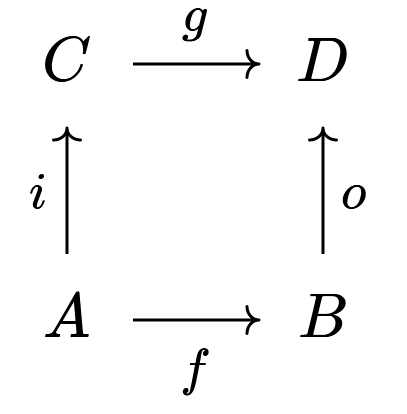
\includegraphics[width=0.25\textwidth]{{./square.png}}

Then the kernel $Ker(d)$ forms a functional dataflow relation of $f$.
\end{theorem}

\begin{proof}
let $a,b$ be elements of $A$ and suppose that $a =_i b$ then $i(a) = i(b)$. Applying $g$ to both sides of this equation yields $g(i(a)) = g(i(b))$. By the commutative diagram above, we have that $g(i(x)) = o(f(x))$ for all $x \in A$ so we can replace $g \circ i$ in these equations with $o \circ f$ to get $o(f(a)) = o(f(b))$. Rewriting this in relational format yields $f(a) =_o f(b)$. So that $a =_i b$ implies that $f(a) =_o f(b)$.
\end{proof}

It follows that every morphism $d$ in $Sets^{\to}$ yields a functional dataflow relation $Ker(d)$ determined by the ordered pair of kernels of the component functions of $d$. In the other direction, we can extract an epimorphism in $Sets^{\to}$ from a functional dataflow relation $(P,Q)$ using the projection morphism $\pi_{(P,Q)}$.

\begin{definition}
let $f: A \to B$ be a function with dataflow relation $(P,Q)$ and quotient function $\frac{f}{(P,Q)}$ then we can define a morphism of functions by $d : (f: A \to B) \to (\frac{f}{(P,Q)} : P \to Q)$ with component projections $\pi_P : A \to P$ and $\pi_Q : B \to Q$.
\end{definition}

The projection mapping takes any $a \in A$ to the unique class in $P$ such that $a \in P$. The quotient function is defined by projection and choice. The application of $\frac{f}{(P,Q)}$ to an equivalence class $C$ in $P$ proceeds by selecting $c \in C$ and then taking $\pi_{Q}(f(c))$. By the definition of functional dataflow relations, $\pi_{Q}(f(c))$ is always equal for any choice of $c \in C$.

\begin{theorem}
the projection mapping defined by definition 2.2.5 is a morphism in $Sets^{\to}$ with diagram:

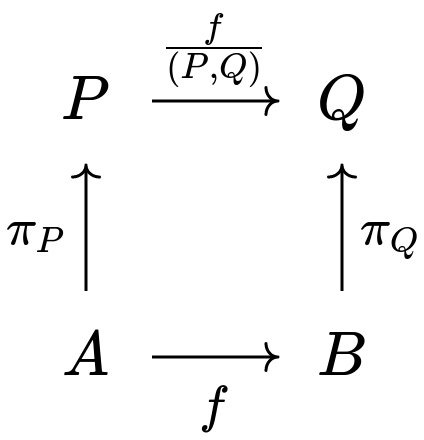
\includegraphics[width=0.25\textwidth]{{./projection.png}}

\end{theorem}

\begin{proof}
let $a \in A$ then we can apply $\pi_Q$ and $f$ to $a$ to get $\pi_{Q}(f(a))$. In the other direction, for a given $a$ the projection $\pi_P$ maps it to an equivalence class $C$ in $P$ that contains it. The quotient $\frac{f}{(P,Q)}$ maps $C$ to $\pi_{Q}(f(c))$ for any choice of a value $c \in C$ and by the definition of functional dataflow relations it produces the same result for any choice including for $a \in C$. It follows that $\pi_{Q}(f(c)) = \pi_{Q}(f(a))$ for any $c \in P$ so that $\frac{f}{(P,Q)} \circ \pi_P$ and $\pi_Q \circ f$ coincide.
\end{proof}

Given an epimorphism class with representative $d$ in $Sets^{\to}$ we can form an ordered pair of partitions by $Ker(d)$. Given an ordered pair of partitions $(P,Q)$ we can produce an epimorphism in $Sets^{\to}$ by $\pi_{(P,Q)}$. It follows that the two concepts coincide.

\subsection{Definition using adjunctions}
In classical set theory, we were introduced to a fundamental adjunction between set images and inverse images determined by the functors $\wp$ and $\wp^{-1}$. A categorically dual adjunction exists between partition images and inverse images.

\begin{definition}
Let $f: A \to B$ be a function and let $P$ be an equivalence relation on $A$. Then the partition image $f(P)$ is the equivalence relation closure $cl(R)$ of the image relation $\{(a,b) : \exists x,y : f(x) = a, f(y) = b \}$.
\end{definition}

\begin{definition}
Let $f: A \to B$ be a function and let $Q$ be an equivalence relation on $B$. Then the partition inverse image $f^{-1}(Q)$ is the equivalence relation defined by $\{(a,b) : f(a) =_Q f(b) \}$.
\end{definition}

The partition image and inverse image form monotone maps of partition lattices $f: Part(A) \to Part(B)$ and $f^{-1}: Part(B) \to Part(A)$ such that $f$ is a lower adjoint and $g$ is an upper adjoint of this adjunction. Partition images and inverse images define the minimal and maximal partitions that can be used on either side of a functional dataflow relation, so that leads to our third definition by adjunctions.

\begin{definition}
Let $f: A \to B$ be a function, then $(P,Q)$ is a functional dataflow relation provided that either $P \subseteq f^{-1}(Q)$ or $f(P) \subseteq Q$ where $\subseteq$ is the inclusion of equivalence relations.
\end{definition}

We will now demonstrate the equivalence of the definition using adjunctions to the definition using ordered pairs of partitions.

\begin{theorem} let $f: A \to B$ be a function with $P$ a partition of $A$ and $Q$ a partition of $B$. Then the following three conditions are logically equivalent:

\begin{enumerate}
 \item $\forall a,b: a =_P b \Rightarrow f(a) =_Q f(b)$.
 \item $P \subseteq f^{-1}(Q)$
 \item $f(P) \subseteq Q$
\end{enumerate}

\end{theorem}

\begin{proof}
suppose that $P \subseteq f^{-1}(Q)$ then by definition 2.2.7 the inverse image $f^{-1}(Q)$ is equal to $\{(a,b) : f(a) =_Q f(b)\}$. So by the definition of inclusion, this means that $\forall a,b : a =_P b \Rightarrow f(a) =_Q f(b)$, which is precisely the statement of condition one. So conditions (1) and (2) are logically equivalent. Condition (3) implies condition (1) for consider $(a,b) \in P \Leftrightarrow a =_P b$ then $f(P) \subseteq Q$ implies that $(f(a),f(b)) \in Q \Leftrightarrow f(a) =_Q f(b)$.

Lastly, condition (1) implies condition (3). Suppose that condition (1) is true, then let $R$ be equal to $\{(f(a),f(b)) : a =_P b\}$. Then condition one says that $R \subseteq Q$. $R$ need not be an equivalence relation. However, $f(P)$ is the equivalence closure of $R$, which means that it is the smallest equivalence relation that contains $R$. It follows that if $Q$ is an equivalence relation and it contains $R$ then it must also contain $cl(R)$. Therefore, $f(P) \subseteq Q$ and condition (1) implies condition (3). It follows that all three conditions are equivalent.
\end{proof}

This theorem is the last piece needed to demonstrate the equivalence of our three definitions. We can now speak of functional dataflow relations as defined by equivalence classes of epimorphisms in $Sets^{\to}$, ordered pairs of partitions preserving equality, or by pairs of partitions determined by the adjunction between partition images and inverse images. That partition images and inverse images form an adjunction easily follows.

\begin{corollary}
let $f: A \to B$ be a function then the partition image $f: Part(A) \to Part(B)$ and inverse image $f^{-1} : Part(B) \to Part(A)$ form a monotone Galois connection from $A$ to $B$ with $f$ as a lower adjoint and $f^{-1}$ as an upper adjoint.
\end{corollary}

This corollary demonstrates that partition images and inverse images form an adjunction. Partition images and inverse images are useful as a computational tool for handling functional dataflow relations.

\subsection{Definition using internal relations}
Let $d: (f: A \to B) \to (g: C \to D)$ be a morphism in $Sets^{\to}$. Then we can form the kernel pair of $d$ by pulling the object back upon itself. First, form the product function $f^2$ and its projection morphisms $\pi_1$ and $\pi_2$. Then form the equalizer of $d \circ \pi_1$ and $d \circ \pi_2$ to get an internal relation $R$ on $f$, which represents a functional dataflow relation.

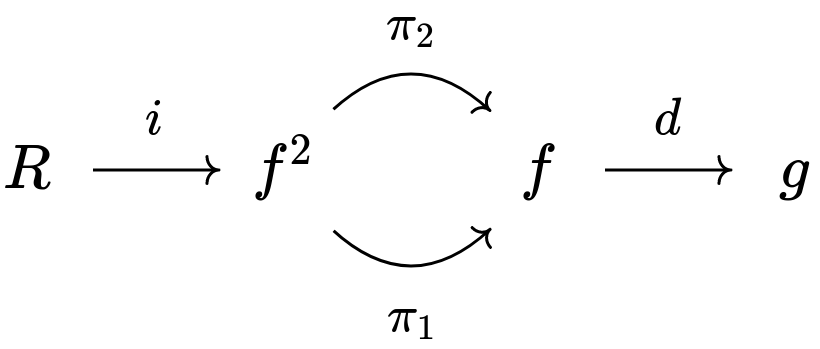
\includegraphics[width=0.50\textwidth]{{./kernelpair.png}}

In the other direction, given a subobject $R$ of $f^2$, we can get its quotient object by forming a coequalizer of $\pi_1 \circ i$ and $\pi_2 \circ i$ to get a projection epimorphism. This demonstrates the equality of this definition with our first definition. By transitivity, this indicates that all four definitions are equivalent.

\begin{itemize}
 \item given an internal dataflow relation $R$ in $Sets^{\to}$ you can form an equivalence class of epimorphisms from it by taking the coequalizer of its projection morphisms
 \item given any equivalence class of epimorphisms in $Sets^{\to}$ that equivalence class can be converted into an internal relation $R$ by taking the pullback of any epimorphism by itself
\end{itemize}

The dataflow model provided by partition adjunctions is essential because it enables more efficient computations. On the other hand, the singular importance of the definition of dataflow relations by internal relations is that we can use it to relate dataflow relations to the logic of $Sets^{\to}$ and its object of truth values $\Omega$.

Let $i: R \to f^2$ be an internal relation of the function $f$. Then by the fact that $Sets^{\to}$ is a topos we can use its subobject classifier to get a characteristic arrow $\chi_i : f^2 \to \Omega$ that classifies $R$ within the subobject lattice of the product function $f^2$.

\[ \chi_i : f^2 \to \Omega \]

Then this equivalent definition of dataflow relations enables us to use logical operators on $\Omega$ on dataflow relations. The logical connectives $and : \Omega^2 \to \Omega$ and $or : \Omega^2 \to \Omega$ recover the lattice operations on dataflow relations. The operation $fill : \Omega \to \Omega$ takes 0 to 0, 1/2 to 1, and 1 to 1 on the inputs of $\Omega$ and is the identity on the outputs. When applied to a functional dataflow relaton $(P,Q)$ it fills it up to produce an injective dataflow relation $(f^{-1}(Q),Q)$. This enables the use of $Sets^{\to}$ logic on dataflow relations.

\section{Duality of set and partition images}
We saw that in $Sets$, there exists a category-theoretic duality of sets and partitions. By transferring settings to the topos $Sets^{\to}$, we now have a category-theoretic duality between set images and partition images.

\begin{itemize}
 \item let $f : A \to B$ be a function with $S \subseteq A$ and $T \subseteq B$ then $(S,T)$ is a subobject of $f$ provided that $f(S) \subseteq T$ or $S \subseteq f^{-1}(T)$.
 \item let $f: A \to B$ be a function with $P$ a partition of $A$ and $Q$ a partition of $B$ then $(P,Q)$ is a quotient object of $f$ provided that $f(P) \subseteq Q$ or $P \subseteq f^{-1}(Q)$.
\end{itemize}

The dual concepts of monomorphisms and epimorphisms in $Sets^{\to}$ can be defined by a dual pair of adjunctions.

\begin{itemize}
 \item let $f: A \to B$ be a function then $\wp(f): \wp(A) \to \wp(B)$ and $\wp(f) : \wp(B) \to \wp(A)$ forms an adjunction between $\wp(A)$ and $\wp(B)$.
 \item let $f: A \to B$ be a function then $Part(f): Part(A) \to Part(B)$ and $Part(f) : Part(B) \to Part(A)$ forms an adjunction between $Part(A)$ and $Part(B)$.
\end{itemize}

The category-theoretic duality between monomorphisms and epimorphisms can be used to infer the duality between set images and partition images in the topos $Sets^{\to}$.

\section{Properties of partition images}

\subsection{Categorical characterization}
Partition images can be defined by coequalizers. Let $f: A \to B$ be a function and let $R$ be an equivalence relation on $A$. Then there exist projections $\pi_1$ and $\pi_2$ on $R$ that map to $A$.

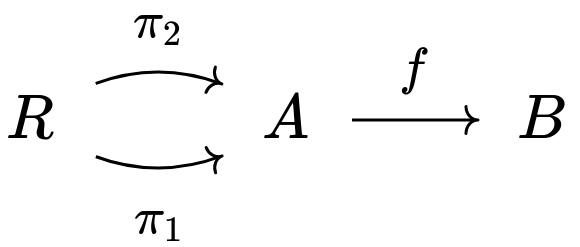
\includegraphics[width=0.30\textwidth]{{./dp.png}}

These produce a composite pair of parallel morphisms on the equivalence relation $R$:

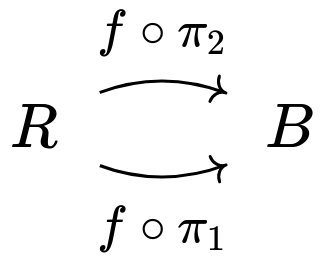
\includegraphics[width=0.18\textwidth]{{./compdiagram.png}}

We can now form the coequalizer of the parallel morphisms $f \circ \pi_1$ and $f \circ \pi_2$ from $P$ to $B$. This produces the following coequalizer diagram in $Sets$.

\newpage

The coequalizer of $f \circ \pi_1$ and $f \circ \pi_2$ is the pair $(Q,q)$ defined by a quotient object and its epimorphism $q: B \to Q$. We canonically identify partitions by equivalence classes of epimorphisms, so the partition on $B$ is isomorphic to the equivalence class of epimorphisms in which $q$ belongs. In other words, the partition on $B$ produced by the partition image on $R$ is equivalent to the kernel $ker(q)$.

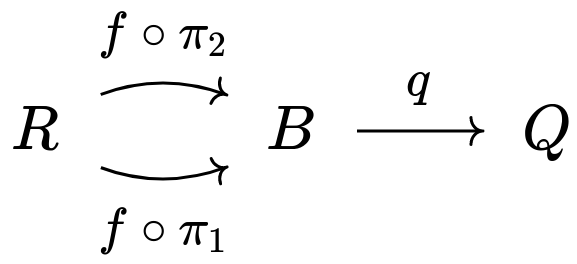
\includegraphics[width=0.35\textwidth]{{./coequalizer.png}}

The coequalizer in $Sets$ takes a parallel pair of morphisms $f: A \to B$ and $g: A \to B$ and it returns the equivalence relation generating by pairs $\{(f(x),g(x)) : x \in A\}$. Then in the case of the parallel pair of morphisms between $R$ and $B$ this yields $\{(f(\pi_1(x,y)), g(\pi_2(x,y)) ) : (x,y) \in P\}$ which can be simplified to $\{(f(x),f(y)) : (x,y) \in P\}$ which is precisely the definition of the equivalence relation generated by the partition image.

The partition inverse image has its own categorically dual characterization using equalizers. Let $f: A \to B$ be a function, $P$ be a partition of $B$, then the function $f$ and the projection $\pi_P$ form the following morphism sequence in $Sets$:

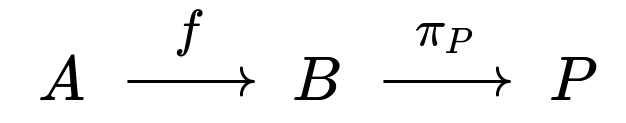
\includegraphics[width=0.30 \textwidth]{{./proj.png}}

Then we can compose these two functions to get $\pi_P \circ f$. Then the partition inverse image of $f$ with respect to $P$ is simply the kernel of $\pi_P \circ f$ denoted $ker(\pi_P \circ f)$. The kernel itself has a categorical characterization using equalizers of diagrams of the following form.

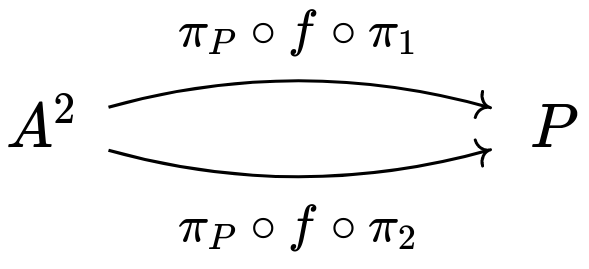
\includegraphics[width=0.30 \textwidth]{{./quad.png}}

Then the equalizer of $\pi_P \circ f \circ \pi_1$ and $\pi_P \circ f \circ \pi_2$ is the pair $(R,r)$ in which $R$ denotes a subobject of $A^2$ which corresponds to an equivalence relation.

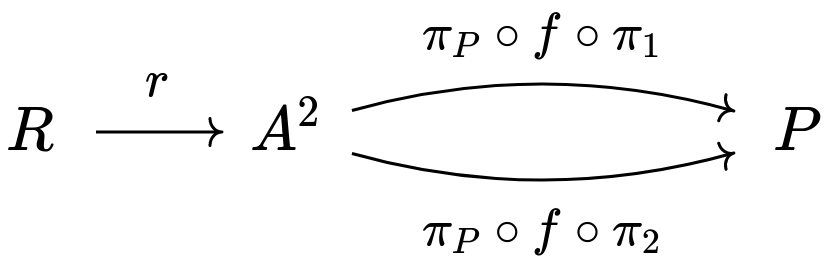
\includegraphics[width=0.45 \textwidth]{{./equalizer.png}}

The equivalence relation $R$ is embedded into $A^2$ by the monomorphism $r$. This characterization is dependent upon the representation of partitions as equivalence relations. To convert $R$ back into a quotient object we can use the coequalizer of its projections, which generates a quotient object for the partition inverse image. Taken together, this demonstrates that equalizers can generate partition images and coequalizers can generate partition inverse images.

\newpage

\subsection{Upper and lower bounds}
Let $Part(A)$ be the partition lattice of a set $A$. Then we will use $A_0$ to denote the lower bound and $A_1$ to denote the upper bound of $Part(A)$.

\begin{definition}
let $A$ be a set then $A_0 = \{(a,b) : a = b\}$ and let $A_1 = A^2$. Then $A_0$ is the equivalence minimal partition of $A$ and $A_1$ is the equivalence minimal partition of $A$.
\end{definition}

Then the partition image and inverse image can be applied to the upper and lower bounds of the partition lattices for any function $f: A \to B$.

\begin{itemize}
 \item $f(A_0) = B_0$ the partition image of the smallest partition produces the smallest partition
 \item $f^{-1}(B_1) = A_1$ the partition inverse image of the largest partition produces the largest partition
 \item $f(A_1)$ the partition image of the largest partition is the image collapsing partition which equates two elements of $B$ provided that they both belong to the image of the function $f$.
 \item $f^{-1}(B_0)$ the partition inverse image of the smallest partition is the kernel of $f$ denoted $=_f$
\end{itemize}

Two special equivalence relations come into focus as a consequence of these applications of the partition image and inverse image function.

\begin{itemize}
 \item $ker(f)$ is the equivalence relation $\{(x,y): f(x) = f(y)\}$
 \item $icp(f)$ is the equivalence relation $\{(x,y) : x \in Im(f) \land y \in Im(f)\}$
\end{itemize}

These two partitions can now be used to establish upper and lower bounds of the partition images and inverse images of a function.

\begin{proposition}
let $f: A \to B$ be a function with $P$ a partition of $A$ and $Q$ a partition of $B$.

\begin{itemize}
 \item $f(P) \subseteq icp(f)$
 \item $ker(f) \subseteq f^{-1}(Q)$
\end{itemize}
\end{proposition}

Of these results, the more interesting of them is that $ker(f) \subseteq f^{-1}(Q)$. This demonstrates that the partition inverse image of a partition $Q$ always produces a partition $f^{-1}(Q)$ which together with $Q$ produces an injective quotient.

\subsection{Lattice theoretic properties}
Let $f: A \to B$ be a function then the partition image and inverse image functions are adjunctions of partition lattices $Part(A)$ and $Part(B)$. This means they have limit/colimit preserving properties common to all adjoints.

\begin{theorem}
partition images are join homomorphisms
\end{theorem}

\begin{proof}
let $f: A \to B$ be a function and let $P$ and $Q$ be partitions of $A$. By the monotonicity of partition images $f(P) \vee f(Q) \subseteq f(P \vee Q)$. It remains to show the converse $f(P \vee Q) \subseteq f(P) \vee f(Q)$. The left-hand side $f(P \vee Q)$ is generated by the image of all pairs in $P \vee Q$. Such a pair $(x,y)$ is determined by a sequence $(x,c_1,...c_n,y)$ of terms that are consecutively $P$-equal or $Q$-equal.

The image of $(x,c_1,...c_n,y)$ under $f$ is $(f(x),f(c_1),...f(c_n),f(y))$. Then each pair in $(x,c_1,...c_n,y)$ is consecutively either $P$-equal or $Q$-equal. It follows that the image $(f(x),f(c_1),...f(c_n),f(y))$ is consecutively either $f(P)$ equal or $f(Q)$ equal so that $f(x)$ is equal to $f(y)$ with respect to $f(P) \vee f(Q)$.

The left-hand side $f(P \vee Q)$ is the minimal equivalence relation generated by all pairs in $P \vee Q$. The relation generated by all pairs in $P \vee Q$ is contained in $f(P) \vee f(Q)$, and $f(P) \vee f(Q)$ is an equivalence relation so it must contain $f(P \vee Q)$. Combining $f(P) \vee f(Q) \subseteq f(P \vee Q)$ with $f(P \vee Q) \subseteq f(P) \vee f(Q)$ yields $f(P \vee Q) = f(P) \vee f(Q)$.
\end{proof}

Partition images are not in general meet homomorphisms. They are meet homomorphisms when the function $f:A \to B$ is injective.

\begin{lemma}
injective relation images preserve transitivity
\end{lemma}

\begin{proof}
let $f: A \to B$ be an injective function and suppose that $R$ is a transitive binary relation on $A$. Let $(x,y) \in f(R)$ and $(y,z) \in f(R)$. There there exist values $a,b,c,d$ such that $(a,b) \in R$, $(x,y) = (f(a),f(b))$, $(c,d) \in R$, and $(y,z) = (f(c),f(d))$.

We have that $f(b) = f(c)$ and since $f$ is injective this implies that $b = c$. Substituting into the previous equations we have $(a,b) \in R$ and $(b,d)$ in $R$. This implies that $(a,d)$ in $R$ and now taking the image with respect to $f$ this yields that $(f(a),f(d)) \in f(R)$ which is the same thing as $(x,z) \in f(R)$. So the image relation $f(R)$ is transitive.
\end{proof}

This lemma aids in the computation of injective partition images.

\begin{corollary}
let $f: A \to B$ be an injective function then the partition image of a partition $P$ can be computed directly from the relation image of $P$ without computing transitive closures.
\end{corollary}

\begin{theorem}
partition images of injective functions are meet homomorphisms
\end{theorem}

\begin{proof}
by the monotonicity of partition images $f(P \cap Q) \subseteq f(P) \cap f(Q)$. We want to show that $f(P) \cap f(Q) \subseteq f(P \cap Q)$. Let $(b_1,b_2) \in f(P) \cap f(Q)$. Then by corollary 2.4.1 there exists $(g_1,g_2) \in P$ and $(h_1,h_2) \in Q$ such that $(f(g_1),f(g_2)) = (b_1,b_2)$ and $(f(h_1),f(h_2)) = (b_1,b_2)$. By the fact that $f$ is injective this implies that $(g_1,g_2) = (h_1,h_2)$. It follows that $(g_1,g_2) = (h_1,h_2) \in P \cap Q$. Then since $(g_1,g_2) \in P \cap Q$ and $(b_1,b_2) = (f(g_1),f(g_2))$ this implies that $(b_1,b_2) \in f(P \cap Q)$. It follows that $f(P) \cap f(Q) \subseteq f(P \cap Q)$.
\end{proof}

\begin{corollary}
partition images of injective functions are lattice homomorphisms
\end{corollary}

\begin{theorem}
let $f : A \to B$ be an injective function then $Part(f): Part(A) \to Part(B)$ is the lattice embedding that embeds $Part(A)$ into the principal down set generated by $icp(f)$.
\end{theorem}

\begin{proof}
$f: A \to B$ is an injective function so it has an underlying bijection $f: A \to Im(f)$. Then since this is a bijection, it produces a bijection between partition lattices $Part(A) \to Part(Im(f))$. Any partition in $Part(Im(f))$ can then be extended to partition on $Part(B)$ by adding on all non-image elements as distinguished members.

Then this mapping from $Part(Im(f))$ to $Part(B)$ is an injection, and so by composition the produced mapping from $Part(A)$ to $Part(B)$ defined by partition images is also injective. As the image of this extension mapping is all the image collapsing partitions, which are partitions that are contained in $icp(f)$, it follows that the partition image function embeds $Part(A)$ into the principal down set generated by $icp(f)$.
\end{proof}

\begin{theorem}
partition inverse images are meet homomorphisms
\end{theorem}

\begin{proof}
let $f: A \to B$ be a function then by definition $f^{-1}(P \cap Q) = \{(x,y) : f(x) =_P f(y) \land f(x) =_Q f(y) \}$. This can be turned into an intersection $\{(x,y) : f(x) =_P f(y) \} \cap \{(x,y) : f(x) =_Q f(y)\}$. Then by expressing this again in terms of inverse images we get $f^{-1}(P) \cap f^{-1}(Q)$. It follows that $f^{-1}(P \cap Q) = f^{-1}(P) \cap f^{-1}(Q)$ which implies that $f$ is a meet homomorphism.
\end{proof}

\begin{theorem}
partition inverse images of surjective functions are join homomorphisms
\end{theorem}

\begin{proof}
let $f: A \to B$ be a function with $P$ and $Q$ partitions of $B$. Let $a_1,a_2 \in A$ then for $a_1 =_{f^{-1}(P \vee Q)} a_2$ to be the case this implies that $f(a_1) =_{P \vee Q} f(a_2)$. In other words, there is a sequence $(f(a_1),b_1,...b_n,f(a_2))$ in $B$ such that each term is consecutively $P$ equal or $Q$ equal. We have that $f$ is surjective, so each of these terms in this sequence has at least one inverse image.

Select a choice of fibers from this sequence $(a_1,b_1',...b_n',a_2)$. Then pairs in $(a_1,b_1',...b_n',a_2)$ are consecutively either $f(P)$ or $f(Q)$ equal so this implies that $a_1$ is equal to $a_2$ with respect to $f^{-1}(P) \vee f^{-1}(Q)$. It follows that $a_1 = _{f^{-1}(P) \vee f^{-1}(Q)} a_2$ so that $f^{-1}(P \vee Q) \subseteq f^{-1}(P) \vee f^{-1}(Q)$. The reverse inclusion holds by the monotonicity of partition inverse images, so $f^{-1}(P \vee Q) = f^{-1}(P) \vee f^{-1}(Q)$.
\end{proof}

\begin{corollary}
partition inverse images of surjective functions are lattice homomorphisms
\end{corollary}

\begin{theorem}
let $f : A \to B$ be an injective function then $Part(f): Part(A) \to Part(B)$ is the lattice embedding that embeds $Part(B)$ into the principal upper set generated by $ker(f)$.
\end{theorem}

\begin{proof}
let $P$ be the set of equivalence classes on $ker(f)$, then any partition on $P$ generates an equivalence relation on $A$ by taking the union of all members of equivalence classes in $P$ contained in an equivalence class in $A$. Each of the resulting union equivalence relations is bigger than $ker(f)$ as they are contained by equating its members by the equivalence relation on $P$. This produces a natural mapping between $Part(Q)$ and the principal upper set generated by $ker(f)$.

We will see that the partition inverse image can be made to filter through this function from $Part(Q) \to Part(B)$. There is a bijective mapping that maps any set on $B$ to a set on $Q$ by taking fibers. So it follows that this maps any partition on $B$ to a partition on $Q$ by the same process. Then by filtering through the inflation of $Q$ partitions into $A$ partitions, this produces an injective embedding of $Part(B)$ into the principal upper set generated by $ker(f)$.
\end{proof}

If $f: A \to B$ is a function then $Part(f): Part(A) \to Part(B)$ and $Part^{-1}(f) : Part(B) \to Part(A)$ both are functions whose kernels and images have been fully characterized. In both cases, the kernels and images of the partition image and inverse image functions are described using the partitions $ker(f)$ and $icp(f)$.

\begin{itemize}
 \item let $f: A \to B$ be a function then $ker(Part(f))$ has that $P$ is equal to $Q$ provided that $P \vee ker(f) = Q \vee ker(f)$. The image of $f$ is all partitions on $B$ that are less than $icp(f)$.
 \item let $f: A \to B$ be a function then $ker(Part^{-1}(f))$ has that $P$ is equal to $Q$ provided that $P \cap icp(f) = Q \cap icp(f)$. The image of $Part^{-1}(f)$ is all partitions on $A$ that are greater than $ker(f)$.
\end{itemize}

Let $f: A \to B$ be a function, then $Part(f): Part(A) \to Part(B)$ and $Part(f)^{-1}: Part(B) \to Part(A)$ are adjoints of one another. As is the case for every monotone Galois connection, $Part(f)$ and $Part(f)^{-1}$ are associated to a closure operator $f^{-1} \circ f$ and an interior operator $f \circ f^{-1}$. These closure and interior operators on partition lattices are discussed next.

\newpage

\subsection{Closure and interior operators}

Let $f: A \to B$ be a function then for any given partition $P$ representing some set of bits of information, then that partition determines a specific collection of bits of information in the output denoted $f(P)$. However, the lossy nature of an irreversible function $f$ means that the same output collection of information may be determined by some subset of the bits of information in $P$.

This leads to the notion of the injective equivalence closure $f^{-1}(f(P))$. The injective equivalence closure takes a given piece of information in the input, and it determines the minimal subset of information needed to determine the functions partition output. So for example, $f^{-1}(f(A_0))$ is equal to the kernel of $f$.

\begin{definition}
let $f: A \to B$ be a function with $P$ a partition of $A$. Then the injective equivalence closure of $P$ is $f^{-1}(f(P))$.
\end{definition}

The interior operator of the partition adjunction $f \circ f^{-1}$ on the other hand deals with the relationship between the partition image and the set image of a function $Im(f)$. As the partition image is determined by the applications of the function $f$ it can only ever equate elements of the image of the function.

\begin{definition}
let $f:A \to B$ be a function with $Q$ a partition of $B$. Then the image equivalence interior of $Q$ is $f(f^{-1}(Q))$.
\end{definition}

The following special identities make it easy to compute the closure and interior operators of the partition adjunction.

\begin{theorem}
let $f: A \to B$ be a function with $P$ a partition of $A$ and $Q$ a partition of $B$ then

\begin{enumerate}
 \item $f^{-1}(f(P)) = P \vee ker(f)$
 \item $f(f^{-1}(Q)) = Q \cap icp(f)$
\end{enumerate}

\end{theorem}

\begin{proof}
(1) let $(a,b) \in P$ then $f^{-1}(f(a,b))$ is the set $f^{-1}(a) \times f^{-1}(b)$ which is the cartesian product of the fibers of $a$ and $b$. Then relations of the form $f^{-1}(a) \times f^{-1}(b)$ generate $f^{-1}(f(P))$. Let $(x,y) \in f^{-1}(a) \times f^{-1}(b)$ then $(x,a,b,y)$ is a sequence with the first pair of terms equal by $f$, the second equal by $P$, and the third equal by $f$ again so $x$ and $y$ are then equal by $ker(f) \vee P$. Thusly, $f^{-1}(f(P)) \subseteq P \vee ker(f)$. The dual inclusion holds by the properties of closures and the bounds on partition images.

(2) let $(a,b)$ be elements of the image of $f$ such that $a$ and $b$ are $Q$ equal. Then they have fibers $(x,y)$ such that $f(x) = a$ and $f(y) = b$. Then $(x,y)$ is in $f^{-1}(Q)$ and furthermore $(a,b)$ is in $f(f^{-1}(Q))$. So $Q \cap icp(f) \subseteq f(f^{-1}(Q))$. The dual inclusion holds by the properties of interiors and the bounds on partition inverse images.
\end{proof}

The dual operators of closure and interior $f \circ f^{-1}$ and $f^{-1} \circ f$ of the partition adjunction produce important fixed points.

\begin{itemize}
 \item the fixed points of $f^{-1} \circ f$ are the kernel preserving partitions
 \item the fixed points of $f \circ f^{-1}$ are the image collapsing partitions
\end{itemize}

By theorem 2.4.5 it is not hard to see that these fixed points are both sublattices in their respective input and output partition lattices, and not only that, they are principal up or down sets.

\begin{corollary}
let $f: A \to B$ be a function then

\begin{itemize}
 \item the kernel preserving partitions form a principal upper set of $Part(A)$
 \item the image collapsing partitions form a principal down set of $Part(B)$.
\end{itemize}
\end{corollary}

Every monotone Galois connection is associated with fixed points in its source set and target set. In the case of the partition adjunction, these fixed points are the kernel-preserving partitions and the image-collapsing partitions.

\subsection{Functorial properties}
Let $Sets$ be the topos of sets. Then corresponding to the adjunction between partition images and partition inverse images is the dual pair of functors: the covariant functor $Part$ and the contravariant functor $Part^{-1}$.

\[ Part : Sets \to Sets \]
\[ Part^{-1} : Sets \to Sets \]

These could also be defined by functors to the category $Ord$ of partial orders and monotone maps. In other cases, they might be functors to categories of residuated or coresiduated maps. We will prove that these mappings define valid functors.

\begin{theorem}
$Part(f \circ g) = Part(f) \circ Part(g)$
\end{theorem}

\begin{proof}
the partition image is a join homomorphism, so it maps generating systems for equivalence relations to generating systems. Therefore, $f \circ g$ of $P$ is the equivalence relation generated by $\{(f(g(x)),f(g(y))\}$ with $x =_P y$. $g$ of $P$ is $\{(g(x),g(y)) : x =_P y \}$ and so applying $f$ to it yields $\{(f(g(x)),f(g(y))\}$. Therefore, $(f \circ g)(P) = f(g(P))$ and the two equations coincide. It follows the partition image mapping is functorial.
\end{proof}

\begin{theorem}
$Part^{-1}(f \circ g) = Part^{-1}(g) \circ Part(f)$
\end{theorem}

\begin{proof}
let $P$ be a partition and consider $Part^{-1}(f \circ g)(P)$ then this is equal to $\{(x,y) : f(g(x)) =_P f(g(y))\}$. Consider on the other hand, $Part^{-1}(g)(Part^{-1}(f)(P))$ then we can expand $Part^{-1}(f)(P)$ in this expression to get $Part^{-1}(g)(\{(x,y) : f(x) =_P f(y)\}$. Further expanding $Part^{-1}(g)$ yields $\{(x,y) : (g(x),g(y)) \in \{(x,y) : f(x) =_P f(y)\}\}$. This can be simplified to $\{(x,y) : f(g(x)) = f(g(y))\}$.
\end{proof}

The compositionality of the partition image and inverse images is helpful if you want to algorithmically compute partition images and inverse images for a given function. With these theorems, the computation of specific  partition images and inverse images can be simplified by decomposing a function into simpler functions using function composition in $Sets$.

\subsection{Relations generated by partition images}
The partition image and inverse image functions define dataflow relations for each argument partition they receive. These dataflow relations have a special role to play.

\begin{itemize}
 \item let $f: A \to B$ be a function and let $P$ be a partition of $f$ then a dataflow relation of the form $(P,f(P))$ is called a full relation on $f$.
 \item let $f: A \to B$ be a function and let $Q$ be a partition of $f$ then a dataflow relation of the form $(f^{-1}(Q),Q)$ is called an injective relation on $f$.
\end{itemize}

In a few exceptional cases, they coincide. The fixed points of the composed operators form special classes of partitions in $A$ and $B$. In the first case, $f^{-1} \circ f$ has as fixed points all partitions $P$ such that $ker(f) \subseteq P$. In the second case, $f \circ f^{-1}$ has as fixed points all partitions $Q$ such that $Q \subseteq icp(f)$.

If $P$ is a fixed point of $f^{-1} \circ f$ then it is the case that $(P,f(P)$ is also an injective congruence for $(f^{-1}(f(P)), f(P)) = (P,f(P))$. Dually, if $Q$ is a fixed point of $f \circ f^{-1}$ then $(f^{-1}(Q), f(f^{-1}(Q))) = (f^{-1}(Q), Q)$ so that $(f^{-1}(Q),Q)$ is a full congruence.

\begin{itemize}
 \item let $f: A \to B$ be a function and let $(P,Q)$ be a congruence of $f$ then $(P,Q)$ is both a full and an injective congruence provided that $P$ and $Q$ are fixed points of the closure operators of the partition adjunction on their respective sets.
\end{itemize}

Using the logical operator $fill : \Omega \to \Omega$ defined on the object of truth values $\Omega$ of the topos $Sets^{\to}$ the injective dataflow relations $(f^{-1}(Q),Q)$ can equivalently be considered to be those that are generated by the use of the method $fill : \Omega \to \Omega$ on their expression as internal relations. Fill takes any dataflow relation and it makes it injective, by filling up the input with any missing equal pairs.

\newpage

\section{Operations on functional dataflow relations}
The division of memory into places and locations is handled by partition logic. All computations that move around data from one place to another are modeled using functional dataflow relations. As the core concept of our model of computation, a number of different operations have been defined on them.

\begin{itemize}
 \item composition
 \item restriction
 \item partition
 \item quotients
 \item join/meet
 \item products/coproducts
 \item preservation/reflection
 \item morphisms
\end{itemize}

In order to create a good general idea of functional dataflow relations, we will review each of these different operations and their properties. As we will be using these relations as the means by which we logically reason about computation, any theorems we can prove about them will be helpful.

\subsection{Quotients}
We can form quotients of functions by dataflow relations in $Sets^{\to}$.

\begin{definition}
let $f: A \to B$ be a function with $(P,Q)$ a congruence of $f$. Then we define the quotient $\frac{f}{(P,Q)}$ to be the function which maps any equivalence class in $P$ to the unique equivalence class in $Q$ that all of its members are mapped to. Let $C$ be an equivalence class in $P$ then given a choice $c \in C$ this can be defined by $\pi_Q(c)$.
\end{definition}

There also exists a corresponding projection epimorphism $\pi_{(P,Q)} : f \to \frac{f}{(P,Q)}$ in $Sets^{\to}$ whose existence is guaranteed by theorem 2.2.2. Quotients can be used to classify the congruences of a function into special classes.

\begin{definition}
let $f$ be an object in $Sets^{\to}$ then an injective congruence of $f$ is a pair $(P,Q)$ for whom the quotient $\frac{f}{(P,Q)}$ is injective.
\end{definition}

\begin{theorem}
let $f: A \to B$ then the injective congruences of $f$ are all congruences of the form $(f^{-1}(Q),Q)$ for some $Q$ in $Part(b)$.
\end{theorem}

\begin{proof}
every function preserves equality $a = b \Rightarrow f(a) = f(b)$. An injective function also reflects equality so that $f(a) = f(b) \Rightarrow a = b$. Taken together this means that $a = b \Leftrightarrow f(a) = f(b)$. If we take this approach to definition two of a functional congruence relation then $a =_P b \Rightarrow f(a) =_Q f(b)$ becomes $a =_P b \Leftrightarrow f(a) =_Q f(b)$. Then in that case $a =_P b$ is equal to the relation $\{(a,b) : f(a) =_Q f(b)$ which is precisely $f^{-1}(Q)$.
\end{proof}

\begin{definition}
let $f$ be an object of $Sets^{\to}$ then a surjective congruence of $f$ is a pair $(P,Q)$ for which the quotient $\frac{f}{(P,Q)}$ is surjective.
\end{definition}

The property that a given congruence is surjective has its own special characterisation. It is clear from this alternate definition that a congruence $(P,Q)$ is a surjective congruence if and only if its $Q$ partition equalizes non-images with images.

\begin{proposition}
let $f: A \to B$ be a function and let $(P,Q)$ be a congruence of $f$. Let $X = B - Im(f)$ be the non-image of the function $f$ consisting of all elements of $B$ with empty inverse images. Then $(P,Q)$ is a surjective congruence provided that for every equivalence class $C$ in $Q$ we have $C \not\subseteq X$.
\end{proposition}

\begin{theorem}
let $f: A \to B$ be a surjective function and let $(P,Q)$ be a congruence of $f$ then $\frac{f}{(P,Q)}$ is surjective.
\end{theorem}

\begin{proof}
let $C$ be an equivalence class in $Q$ then as $f$ is surjective every element in $B$ has fibers. Let $c$ be a choice of an element in $C$ then it has a fiber $f^{-1}(c)$ in $A$. This fiber has at least one element $x$ that maps to $c$, so given that $x$ we can construct a fiber for $Q$ in $\frac{f}{(P,Q)}$ of the form $\pi_{P}(x)$. As every element of $Q$ has a fiber in $P$, the quotient function is surjective.
\end{proof}

\begin{theorem}
let $f: A \to B$ be a function and let $(P,Q)$ be a surjective congruence of $f$. Let $(R,S)$ be another congruence of $f$ that is more equal then $(P,Q)$ so that $P \subseteq R$ and $Q \subseteq S$. Then $(R,S)$ is a surjective congruence.
\end{theorem}

\begin{proof}
let $X$ be the set of all elements of $B$ with empty fibers. Then by proposition 2.5.1 we have that for each equivalence class $C$ in $Q$ it is the case that $C \not\subseteq X$. We also have that $Q \subseteq S$ which implies that for each equivalence class $D$ in $Q$ it is the case that there exists some $C$ in $Q$ such that $C \subseteq D$. Now since $C \not\subseteq X$ and $C \subseteq D$ we have that $D \not\subseteq X$.
\end{proof}

\subsection{Composition}
Functional dataflow relations in $Sets^{\to}$ can be composed with one another.

\begin{theorem}
let $f: A \to B$ and $g: B \to C$ be functions with $(P,Q)$ a functional dataflow relation on $f$ and $(Q,R)$ a functional dataflow relation on $g$. Then $(P,R)$ is a functional dataflow relation on $g \circ f$.
\end{theorem}

\begin{proof}
let $a,b \in A$ and suppose that $a =P b$ then since $f$ maps $P$ equal terms to $Q$ equal ones this implies that $f(a) =_Q f(b)$. Now since $g$ maps $Q$ equal terms to $R$ equal ones this implies that $g(f(a)) =_R g(f(b))$. It follows that $a =_P b \Rightarrow g(f(a)) =_R g(f(b))$ so that $(P,R)$ is a functional dataflow relation for $g \circ f$.
\end{proof}

This leads to a form of categorical semantics for functional dataflow relations, wherein they are morphisms in the category $Setoids$.

\begin{theorem}
let $f: A \to B$ and $g: B \to C$ be functions with $(P,Q)$ a functional dataflow relation of $f$ and $(Q,R)$ a functional dataflow relation on $g$. Then quotients preserve composition $\frac{g}{(Q,R)} \circ \frac{f}{(P,Q)} = \frac{g \circ f}{(P,R)}$.

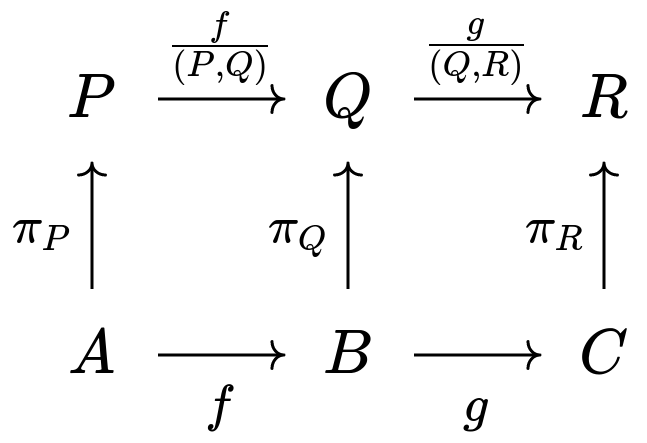
\includegraphics[width=0.4\textwidth]{{./quotcomp.png}}
\end{theorem}

\begin{proof}
let $C$ be an equivalence class of $P$ and let $c \in C$ be a choice of $C$ then $\frac{g \circ f}{(P,R)}(C) = \pi_R(g(f(c))$. By comparison, $\frac{f}{(P,Q)} = \pi_Q(f(c))$ so then applying $\frac{g}{(Q,R)}$ to it will require us to take a value $d$ that is $Q$ equal to $f(c)$ and then computing $\pi_R(d)$ but $g$ maps $Q$ equal terms to $R$ equal ones so $\pi_R(d) = \pi_R(g(f(c)))$ and the two values coincide.
\end{proof}

Let $C$ be a category then if $C$ is $Setoids$-enriched this is equivalent to $C$ having an arrow congruence defined on it. In that case, $C$ is associated with a quotient category $Quot(C)$. It happens that $Setoid$ is self-enriched by componentwise comparisons.

\begin{definition}
let $Setoid$ be the category of setoids. Then it is self-enriched with equivalence relation on $Hom(P,Q)$, $P \subseteq A^2, Q \subseteq B^2$ defined by equating $f: P \to Q$ and $g: P \to Q$ provided that $\forall x \in A : f(x) =_Q g(x)$.
\end{definition}

Then the equivalence relations on the hom classes of Setoid are equivalent to quotient equivalence. In other words, $f$ and $g$ are equal in $Hom(P,Q)$ provided that $\frac{f}{(P,Q)} = \frac{f}{(P,Q)}$. With this construction, we see that the quotient category of the category of setoids enriched in itself is simply the category of $Sets$ which is defined by the quotient functor. The quotient functor takes any setoid to its quotient set and any morphism of setoids to its quotient function.

\[ Quot : Setoid \to Sets \]

This quotient functor is inherently associated to the category of setoids by its self-enrichment.

\subsection{Meet and join}
Functional dataflow relations form a lattice by its meet and join operations. The meet operation has an intuitive interpretation: if the data in memory location $A$ determines the data in location $B$ and the data in location $C$ determines the data in location $D$, then the combined data in both $A$ and $C$ determines the combined data in $B$ plus $D$.

\begin{theorem}
let $f: A \to B$ be a function and let $(P_1,Q_1)$ and $(P_2,Q_2)$ be congruences of $f$ then $(P_1 \cap P_2, Q_1 \cap Q_2)$ is a congruence of $f$.
\end{theorem}

\begin{proof}
suppose that $a =_{P_1 \cap P_2} b$ then $a =_{P_1} b$ and $a =_{P_2} b$. Then by the fact that $a =_{P_1} b$ and $(P_1, Q_1)$ is a congruence we have that $f(a) =_{Q_1} f(b)$. Furthermore, since $a =_{P_2} b$ and $(P_2,Q _2)$ is a congruence we have that $f(a) =_{Q_2} f(b)$.Now by combination $f(a) =_{Q_1 \cap Q_2} f(b)$. So $(P_1 \cap P_2, Q_1 \cap Q_2)$ is a congruence of $f$.
\end{proof}

The join operation on function congruences states the data in common between $A$ and $B$ produces the data in common between $C$ and $D$ when $(A,C)$ and $(B,D)$ are congruences.

\begin{theorem}
let $f: A \to B$ be a function and let $(P_1, Q_1)$ and $(P_2, Q_2)$ be congruences of $f$ then $(P_1 \vee P_2, Q_1 \vee Q_2)$ is a congruence of $f$.
\end{theorem}

\begin{proof}
by the third definition of functional dataflow relations, the condition that $(P_1 \vee P_2, Q_1 \vee Q_2)$ is a congruence is equivalent to the condition that $f(P_1 \vee P_2) \subseteq (Q_1 \vee Q_2)$. By the fact that partition images are join homomorphisms $f(P_1 \vee P_2) = f(P_1) \vee f(P_2)$.

We can use the third definition of functional dataflow relations to express that $(P_1,Q_1)$ and $(P_2,Q_2)$ are congruences as $f(P_1) \subseteq Q_1$ and $f(P_2) \subseteq Q_2$. The join operation is monotone and increasing so $f(P_1) \subseteq Q_1 \vee Q_2$ and $f(P_2) \subseteq Q_1 \vee Q_2$.

It follows that $Q_1 \vee Q_2$ is an upper bound of $f(P_1)$ and $f(P_2)$. Now since $f(P_1) \vee f(P_2)$ is the least upper bound of $f(P_1)$ and $f(P_2)$ it must be the case that $f(P_1) \vee f(P_2) \subseteq Q_1 \vee Q_2$. By the third definition of functional dataflow relations this implies that $(P_1 \vee P_2, Q_1 \vee Q_2)$ is a function congruence.
\end{proof}

Using these two join and meet operations, we can construct a congruence lattice for a function $f$ denoted $Con(f)$.

\begin{definition}
let $f: A \to B$ be a function and let $Con(f)$ be the set of congruences of $f$. Define the join and meet on $Con(f)$ by:
\begin{itemize}
 \item $(P_1,Q_1) \cap (P_2,Q_2) = (P_1 \cap P_2, Q_1 \cap Q_2)$.
 \item $(P_1,Q_1) \vee (P_2, Q_2) = (P_1 \vee P_2, Q_1 \vee Q_2)$.
\end{itemize}

Then $(Con(f), \cap, \vee)$ forms a lattice: the lattice of congruences of the function $f$.
\end{definition}

Theorems 2.5.3 and 2.5.4 demonstrate that the meet and join operations of $Con(f)$ for a function $f:A \to B$ are inherited from the componentwise meet and join operations in the lattice of partitions $Part(A)$ and $Part(B)$.

\begin{corollary}
let $f: A \to B$ be a function then $Con(f)$ is a sublattice of $Part(A) \times Part(B)$.
\end{corollary}

The category-theoretic dual statement to this is that the lattice of subobjects of a function $f: A \to B$ is a sublattice of $\wp(A) \times \wp(B)$ by which it follows that $\wp(A) \times \wp(B)$ is distributive. The fact that $Con(f)$ is embedded in a partition lattice doesn't produce any similarly interesting results because the generality of partition lattices [5].

As $Con(f)$ is a sublattice of $Part(A) \times Part(B)$ it is associated with dual closure and interior operators. These operators can be constructed by using the adjunction between partition images and inverse images.

\begin{itemize}
 \item the interior of $(P,Q)$ is $(P \cap f^{-1}(Q),Q)$.
 \item the closure of $(P,Q)$ is $(P, Q \vee f(P)$.
\end{itemize}

For small functions $f: A \to B$, it is possible to generate all congruences of the function $Con(f)$ by enumerating partitions and using partition images or inverse images.

\begin{itemize}
 \item let $f : A \to B$ be a function then in order to enumerate all the congruences of $f$ we can first get all partitions of $A$ then for each partition $P$ in $Part(A)$ generate the list of all partitions greater than $f(P)$ in $Part(B)$. Apply concatenate to all these lists to get $Con(f)$.
 \item let $(P,Q)$ be a congruence of $f: A \to B$ then the congruences $(R,S)$ that cover $(P,Q)$ are precisely all congruences generated by equating a pair in $Q$ or by equating a pair in $P$ to get a new partition $P'$ with the property that the new partition image $f(P')$ is still contained in $Q$. Applying this to each congruence in $Con(f)$ generates the covering relation for $Con(f)$.
\end{itemize}

\begin{figure*}[ht!]
\centering
\begin{subfigure}{.5\textwidth}
  \centering
  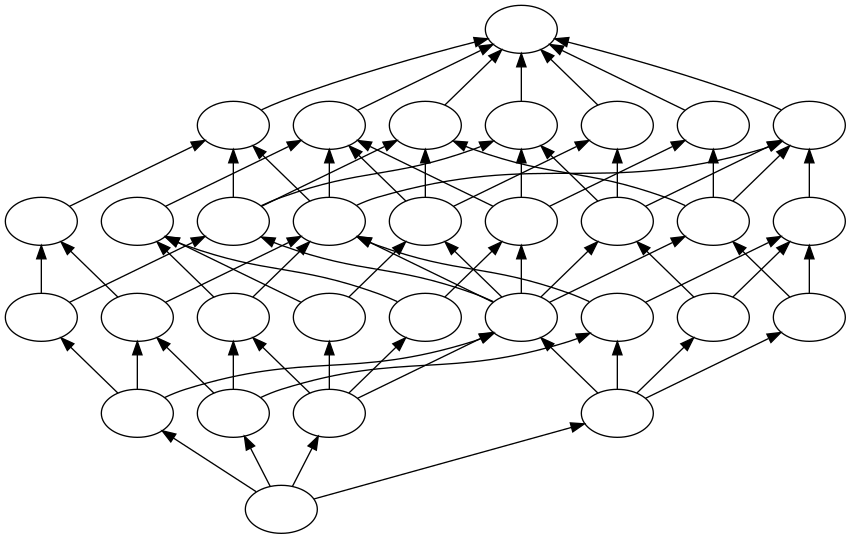
\includegraphics[width=.4\linewidth]{{./cong.png}}
  \caption{Con(f)}
  \label{fig:sub1}
\end{subfigure}%
\begin{subfigure}{.5\textwidth}
  \centering
  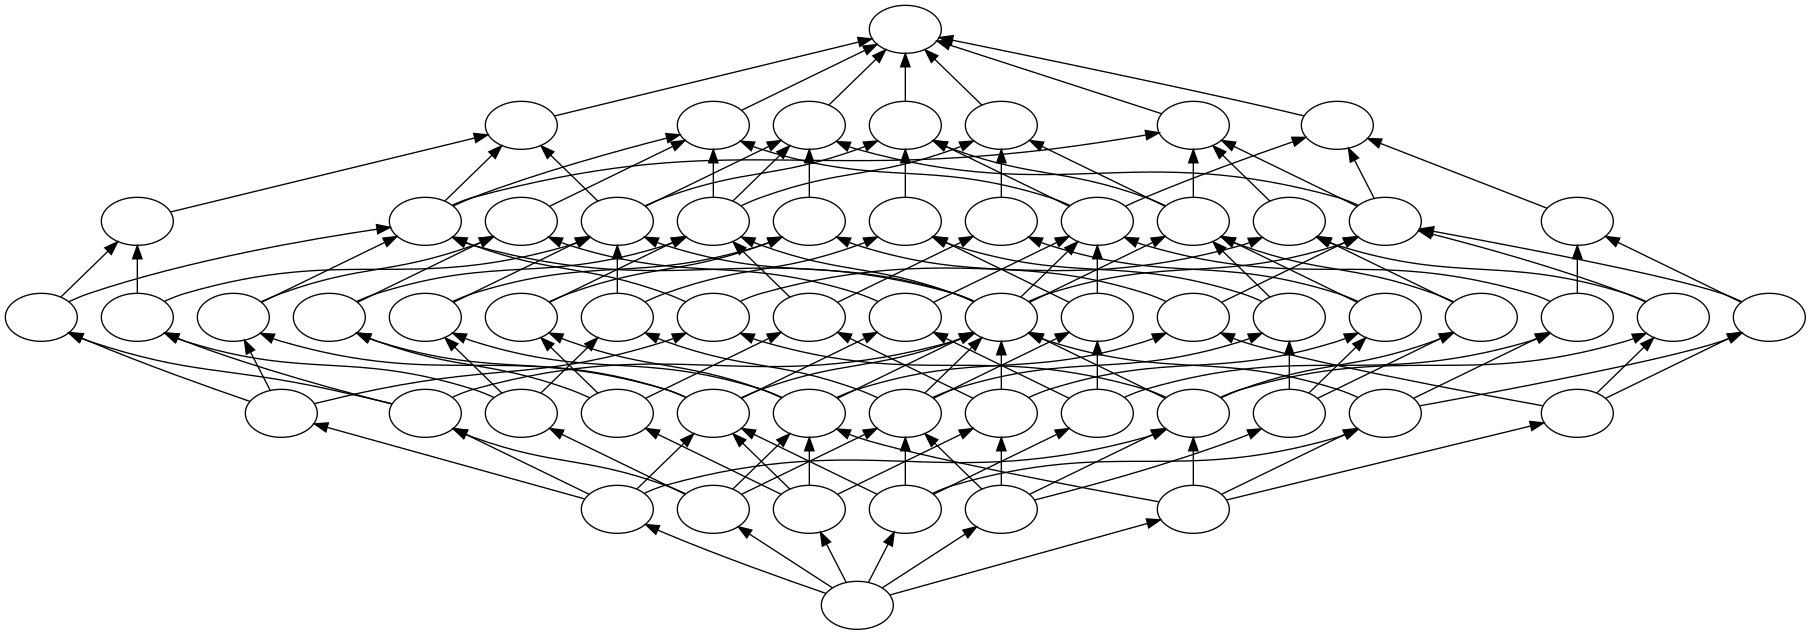
\includegraphics[width=.8\linewidth]{{./conf.png}}
  \caption{Con(f)}
  \label{fig:sub2}
\end{subfigure}
\caption{Congruence lattices of small functions}
\end{figure*}

The join irreducibles and the meet irreducibles in $Con(f)$ have been extensively studied.

\begin{proposition}
let $f: A \to B$ be a function then the join irreducibles in $Con(f)$ are those partitions $(P,Q)$ that belong in one of three classes:
\begin{enumerate}
 \item partitions defined by equating a single pair of elements $b_1,b_2$ in $B$ so that $(A_0,\{b_1,b_2\})$.
 \item partitions defined by equating a pair of elements $a_1,a_2$ in $A$ that are already equalized by $f$ of the form $\{(a_1,a_2),B_0\}$.
 \item partitions defined by the equating a pair of elements $a_1,a_2$ in $A$ that are not equalized by $f$ of the form $\{(a_1,a_2),(f(a_1),f(a_2))$.
\end{enumerate}
\end{proposition}

Of these join irreducibles (1) and (2) are atomic, and (3) depends on a single atom of type (1). The main property of join irreducibles in $Con(f)$ is that they describe how equal pairs in the input transfer into equal pairs in the output.

The meet irreducibles in $Con(f)$ are called functional bitflow relations because they describe how bits of data in the input of a function flow to bits of data in the output. All other functional dataflow relations representing how some set of bits produces another set of bits can be produced from describing how individual bits of information in the input produce bits of information in the output.

\begin{definition}
let $S$ be a set then a bit of information on $S$ is an equivalence relation on $S$ with two equivalence classes.
\end{definition}

\begin{proposition}
let $f: A \to B$ be a function then the meet irreducibles in $Con(f)$ are those partitions $(P,Q)$ that belong in one of three classes:

\begin{enumerate}
 \item partitions defined by a bit of information of $A$ and no information on $B$
 \item partitions defined by a bit of information of $B$ that has no information on the image of $f$ and a partition with no information on $A$
 \item partitions defined by a bit of information of $B$ and the bit of information on $A$ which is its partition inverse image.
\end{enumerate}
\end{proposition}

Of these meet irreducibles (1) and (2) are coatomic. Partitions of type (3) depend upon a single partition of type (1) which is the bit of information in the input that determines the bit of information in the output. The classification of join and meet irreducibles allows us to describe the sort of posets they form in $Con(f)$.

\begin{proposition}
let $f: A \to B$ be a function and $Con(f)$ its congruence lattice
\begin{itemize}
 \item the join irreducibles in $Con(f)$ form a maximum height two lower forest
 \item the meet irreducibles in $Con(f)$ form a maximum height two upper forest
\end{itemize}
\end{proposition}

Of these two the functional bitflow relations are more useful for our model of computation in information systems because they describe how input bits of information determine output bits of information. All other dataflow relations are described as the meet of dataflow relations between bits.

If $f$ is surjective no meet irreducible congruences of type (2) exist and all coatomic congruences are of type (1) and they have no information about the input. All bits of information in the output then reflect back to bits of information in the input, so that bits flow to bits. Our general purpose dataflow model will capture everything from how bits flow to bits to how entire large memory regions flow into other regions.

Next, we can study suborders of the congruence lattices $Con(f)$ of a function $f$. In particular, we can study the suborder of injective congruences in $Con(f)$ and its properties.

\begin{theorem}
let $f: A \to B$ be a function and let $(P,Q)$ and $(R,S)$ be injective congruences of $f$. Then $(P \cap R, Q \cap S)$ is an injective congruence.
\end{theorem}

\begin{proof}
by theorem 2.5.1 we can express $(P,Q)$ as $(f^{-1}(Q),Q)$ and $(R,S)$ as $(f^{-1}(S),S)$. If we now take the intersection of these we get $(f^{-1}(Q) \cap f^{-1}(S), Q \cap S)$. Now by the fact that partition inverse images form a meet homomorphism we have that this is equal to $(f^{-1}(Q \cap S), Q \cap S)$. This implies that $(P \cap R, Q \cap S)$ is an injective congruence.
\end{proof}

\begin{corollary}
let $f: A \to B$ be a function then injective congruences form a meet subsemilattice of $Con(f)$.
\end{corollary}

\begin{theorem}
let $f: A \to B$ be a surjective function and let $(P,Q)$ and $(R,S)$ be injective congruences of $f$. Then $(P \vee R, Q \vee S)$ is an injective congruence.
\end{theorem}

\begin{proof}
by theorem 2.5.1 we can express $(P,Q)$ as $(f^{-1}(Q),Q)$ and $(R,S)$ as $(f^{-1}(S),S)$. We have that $Con(f)$ is a sublattice of $Part(A) \times Part(B)$ so the join of these congruence relations is $(f^{-1}(Q) \vee f^{-1}(S), Q \vee S)$. By the fact that $f$ is surjective the partition inverse image is a join homomorphism so this equals $(f^{-1}(Q \vee S), Q \vee S)$. This implies that $(P \vee R, Q \vee S)$ is an injective congruence.
\end{proof}

\begin{corollary}
let $f: A \to B$ be a surjective function then injective congruences form a sublattice of $Con(f)$
\end{corollary}

This demonstrates the unique role that the injective congruences lattice play within the lattice of congruences of a function. We also have a full characterization of its structure.

\begin{corollary}
let $f: A \to B$ then the lattice of injective congruences of $f$ is isomorphic to $Part(B)$
\end{corollary}

On the other hand, the surjective congruences have the special property that they are upper closed as demonstrated by theorem 2.5.3.

\begin{corollary}
let $f: A \to B$ be a function then the surjective congruences of $f$ form an upper set of $Con(f)$
\end{corollary}

The fact that surjective congruences of $f$ form an upper set means they form a join subsemilattice. Furthermore, that injective congruences form a sublattice when $f$ is surjective means that they form a join subsemilattice too. The intersection of join subsemilattices is a join subsemilattice, so that it follows that bijective congruences form join subsemilattices in the congruence lattices of surjective functions.

\begin{corollary}
let $f: A \to B$ be a function then the bijective congruences of $f$ form an upper subsemilattice of $Con(f)$.
\end{corollary}

Aside from the classification of congruences by their quotients, we considered congruences of the form $(P,f(P))$ as special cases formed by the partition adjunction so we can further examine the role these congruences play in congruence lattices.

\begin{theorem}
let $f: A \to B$ be a function and let $(P_1,f(P_1))$ and $(P_2,f(P_2))$ be congruences of $f$ then $(P_1 \vee P_2, f(P_1) \vee f(P_2))$ is a congruence of $f$
\end{theorem}

\begin{proof}
the partition image function is a join homomorphism so that $f(P_1) \vee f(P_2) = f(P_1 \vee P_2)$. Plug this new value for $f(P_1) \vee f(P_2)$ into the above equation to get $(P_1 \vee P_2, f(P_1 \vee P_2))$ and you can infer that $(P_1 \vee P_2, f(P_1 \vee P_2))$ is a full congruence.
\end{proof}

It follows that the full congruences of the form $(P,f(P))$ form a join subsemilattice of $Con(f)$. As the lower bound $(A_0,B_0)$ is a full congruence the set of full congruences themselves form a lattice embedded in $Con(f)$.

\begin{theorem}
let $f : A \to B$ be a function then the full congruences of $f$ form a join subsemilattice of $Con(f)$
\end{theorem}

With this we have studied all the most important types of congruences in $Con(f)$ for a function $f$ in the topos $Sets^{\to}$.

\subsection{Products and coproducts}
The products and coproducts of function congruences can be defined from the products and coproducts of partitions.

\begin{definition}
let $P$ and $Q$ be equivalence relations then $P+Q$ is equal to $P \cup Q$ if $P$ and $Q$ are disjoint.
\end{definition}

\begin{definition}
let $P$ be an equivalence relation on $A$ and $Q$ an equivalence relation on $B$ then $P \times Q$ is the equivalence relation on $A \times B$ with $((a_1,a_2), (b_1,b_2)) \in P \times Q$ provided that $(a_1,b_1) \in P$ and $(a_2,b_2) \in Q$.
\end{definition}

The topos $Sets^{\to}$ has all limits and colimits. It follows that it has all products and coproducts. To define products and coproducts of dataflow relations we will use the products and coproducts of $Sets^{\to}$ on their underlying functions.

\begin{theorem}
let $f: A \to B$ and $g: C \to D$ be functions with $(P,Q)$ a congruence of $f$ and $(R,S)$ a congruence of $g$. Then $(P \times R, Q \times S)$ is a congruence of $f \times g$.
\end{theorem}

\begin{proof}
let $(a_1,c_1)$ and $(a_2,c_2)$ be equal with respect to $P \times R$ then $a_1 =_P a_2$ and $c_1 =_R c_2$. Then since $(P,Q)$ is a congruence of $f$ we have that $f(a_1) =_Q f(a_2)$ and since $(R,S)$ is a congruence of $g$ we have $g(c_1) =_S g(c_2)$. If we combine $f(a_1) =_Q f(a_2)$ and $g(c_1) =_S g(c_2)$ then we get $(f(a_1),f(a_2))$ and $(g(c_1),g(c_2))$ are equal with respect to $Q \times S$.
\end{proof}

\begin{theorem}
let $f: A \to B$ and $g: C \to D$ be functions with $(P,Q)$ a congruence of $f$ and $(R,S)$ a congruence of $g$. Then $(P + R, Q + S)$ is a congruence of $f + g$.
\end{theorem}

\begin{proof}
let $x$ and $y$ be equal with respect to $P + R$ then either $x$ and $y$ are both in $A$ and $P$ equal in which case they translate to $Q$ equal since $(P,Q)$ is a congruence or they both belong to $C$ and are $R$ equal in which case they translate to $S$ equal values since $(R,S)$ is a congruence. So $P + R$ equal values always produces $Q + S$ equal values with respect to $f + g$.
\end{proof}

These theorems define products and coproducts of function congruences in terms of the topos $Sets^{\to}$. We can further define empty products and coproducts to get the initial and terminal functional dataflow relations.

\begin{itemize}
 \item the empty coproduct congruence is the unique congruence on the initial function $f: \emptyset \to \emptyset$
 \item the empty product congruence is the unique congruence on the terminal function $f: 1 \to 1$
\end{itemize}

The initial object in $Sets^{\to}$ is the function $f: \emptyset \to \emptyset$ and the terminal object is the function $f: 1 \to 1$. In both cases, the initial or terminal congruence can be defined by the unique congruence on the initial or terminal function.

\newpage

\subsection{Preservation and reflection}
Let $d: (f: A \to B) \to (g: C \to D) : (i: A \to C), (o: B \to D)$ be a morphism in the topos $Sets^{\to}$. Then it can be shown that $d$ preserves and reflects function congruences.

\begin{lemma}
let $m: (A,R) \to (B,S)$ be a morphism of directed graphs. Then $m$ preserves transitive closures.
\end{lemma}

\begin{proof}
let $(x,y) \in cl(R)$ then there exists a sequence $(x,c_1,...c_n,y)$ in $R$. Now since $m$ is a homomorphism of directed graphs this produces a sequence $(f(x),f(c_1),...f(c_n),f(y))$ in $S$. It follows that $(f(x),f(y))$ is in $cl(S)$. So $m$ is a homomorphism of digraphs from $(A,cl(R))$ to $(B,cl(S))$
\end{proof}

\begin{corollary} the transitive closure operation $cl: Digraph \to Digraph$ is an endofunctor on the category of digraphs.
\end{corollary}

\begin{lemma}
let $d: (f: A \to B) \to (g: C \to D) : i : A \to C, o : B \to D$ be a morphism of functions. Then $d$ preserves homomorphisms of binary relations.

\end{lemma}

\begin{proof}
let $R$ be a binary relation on $A$ and $S$ a binary relation on $B$ with $f: R \to S$ a homomorphism of binary relations. Then for all $(a,b) \in R$ it holds that $(f(a),f(b)) \in S$. We want to show that $g: i(R) \to o(S)$ is a homomorphism of binary relations.

Suppose that $(a,b)$ is in $i(R)$ this means that there exists $(x,y)$ in $R$ with $i(x) = a$ and $i(y) = b$. We want to show that $(g(a),g(b)) \in o(S)$ which means there exists some $(n,m)$ in $S$ such that $o(n) = g(a)$ and $o(m) = g(b)$. By the fact that $(x,y)$ is in $R$ we have that $(f(x),f(y))$ is in $S$.

As $(f(x),f(y))$ is in $S$, we can use it as a candidate solution for $(n,m)$. Plugging these values in form $(n,m)$ yeilds that $o(f(x)) = g(a)$ and $o(f(y)) = g(b)$. By the fact that $d$ is a morphism in $Sets^{\to}$, it holds that $o \circ f = g \circ i$, so this can be replaced with $g(i(x)) = g(a)$ and $g(i(y)) = g(b)$. As $i(x) = a$ and $i(y) = b$ by supposition, this always holds true. So $g: i(R) \to o(S)$ is a homomorphism of binary relations. This leads to the following diagram in the category of directed graphs:

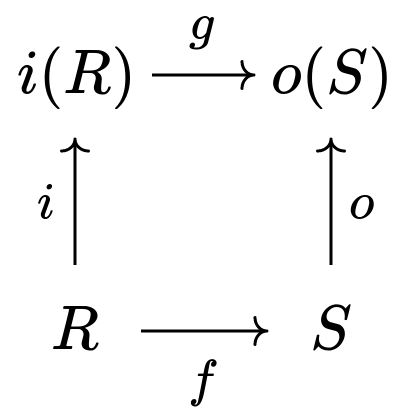
\includegraphics[width=0.20\textwidth]{{./rel.png}}

This diagram is a presheaf of directed graphs with $d$ as its underlying presheaf, which was generated by a binary relation on $f$. As a result, it can be inferred that morphisms in $Sets^{\to}$ preserve homomorphisms of binary relations.
\end{proof}

\newpage

\begin{theorem} let $d: (f: A \to B) \to (g: C \to D) : i : A \to C, o : B \to D$ be a morphism of functions then $d$ preserves function congruences.
\end{theorem}

\begin{proof}
let $(P,Q)$ be a function congruence of $f$ then by lemma 2.5.2 the binary relation images for $P$ and $Q$ form a binary relation homomorphism on $g$ of the form $(i(P),o(Q))$. By lemma 2.5.1 the transitive closures of $i(P)$ and $o(Q)$ again form a homomorphism of binary relations on $Q$, so the partition images $(i(P),o(Q))$ form a function congruence of $g$. This leads to the following presheaf of setoids:

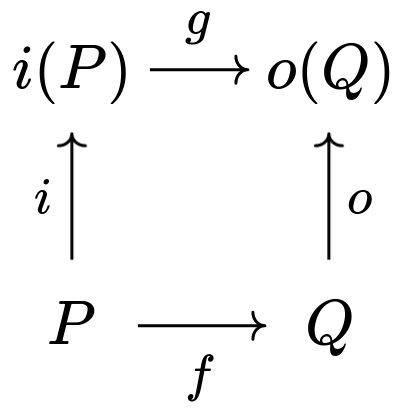
\includegraphics[width=0.20\textwidth]{{./setoid.png}}

It follows that morphisms in $Sets^{\to}$ preserve function congruences so that congruences on $f$ can be mapped to congruences on $g$.
\end{proof}

\begin{theorem} let $d: (f: A \to B) \to (g: C \to D) : i : A \to C, o : B \to D$ be a morphism of functions then $d$ reflects function congruences.
\end{theorem}

\begin{proof}
let $(P,Q)$ be a congruence of $d$ then by theorem 2.2.2 we can form a morphism $\pi_{(P,Q)}$ in $Sets^{\to}$ from the congruence $(P,Q)$ which in turn can be composed with $d$:

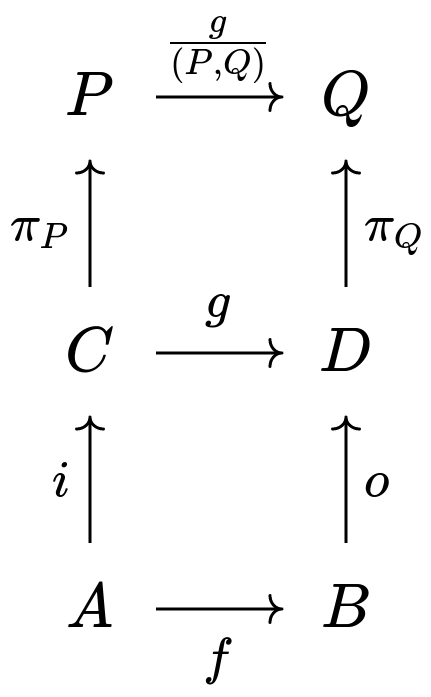
\includegraphics[width=0.2 \textwidth]{{./composite.png}}

Then by theorem 2.2.1 the kernel of the composite $ker(\pi_{(P,Q)} \circ d)$ is a functional dataflow relation of $f$, but this kernel is precisely equal to $(i^{-1}(P),o^{-1}(Q))$ which is the partition inverse image of $(P,Q)$ by $d$. So the morphism $d$ in the topos $Sets^{\to}$ reflects function congruences on $g$ back to function congruences on $f$.
\end{proof}

\newpage

\begin{definition}
let $d: (f: A \to B) \to (g: C \to D) : i : A \to C, o : B \to D$ be a morphism in $Sets^{\to}$ then
\begin{enumerate}
 \item the function congruence image of $(P,Q)$ is $(f(P),f(Q))$
 \item the function congruence inverse image of $(P,Q)$ is $(f^{-1}(P), f^{-1}(Q))$
\end{enumerate}
\end{definition}

The function congruence image / inverse image extends to an adjunction for any morphism $d: f \to g$. The function congruence image is a functor $d: Con(f) \to Con(g)$, and the function congruence inverse image is a functor $d^{-1}: Con(g) \to Con(f)$. Together $d,d^{-1}$ make up an adjunction that generalizes the adjunction between partition images and inverse images to function congruences.

\begin{definition}
let $Sets^{\to}$ be the topos of functions then
\begin{enumerate}
 \item $Con : Sets^{\to} \to Sets$ is the covariant congruence functor on $Sets^{\to}$
 \item $Con^{-1} : Sets^{\to} \to Sets$ is the contravariant congruence functor on $Sets^{\to}$
\end{enumerate}
\end{definition}

 We saw by theorem 2.5.14 and 2.5.15 that congruence images and inverse images are defined componentwise. It follows that they inherit the limit and colimit preserving properties of their partition counterparts.

\begin{corollary}
let $d: (f: A \to B) \to (g: C \to D) : i : A \to C, o : B \to D$ be a morphism in $Sets^{\to}$ then $Con(d) : Con(f) \to Con(g)$ is a join homomorphism and $Con^{-1} : Con(g) \to Con(f)$ is a meet homomorphism
\end{corollary}

The partition adjunction defines two special types of congruences: full congruences $(P,f(P))$ and injective congruences $(f^{-1}(Q),Q)$. These are the two types of congruences that have special behaviour under the congruence adjunction. Full congruences are generated by partition images and preserved by congruence images. Injective congruences are generated by partition inverse images and reflected by congruence inverse images.

\begin{theorem}
let $d: (f: A \to B) \to (g: C \to D) : i : A \to C, o : B \to D$ be a morphism in $Sets^{\to}$ then $d$ preserves full congruences.
\end{theorem}

\begin{proof}
let $(P,f(P))$ be a full congruence of $f: A \to B$. Then the congruence image of $(P,Q)$ under $d$ is $(i(P),o(f(P)))$. The fact that $d$ is a morphism in $Sets^{\to}$ implies that $o \circ f = g \circ i$. Plugging this in to $(i(P),o(f(P)))$ yields $(i(P), g(i(P))$. This implies that $(i(P),g(i(P))$ is the full congruence generated by $i(P)$. As the congruence image of a general full congruence $(P,f(P))$ is again a full congruence it follows that the morphism $d$ preserves full congruences.
\end{proof}

\newpage

\begin{theorem}
let $d: (f: A \to B) \to (g: C \to D) : i : A \to C, o : B \to D$ be a morphism in $Sets^{\to}$ then $d$ reflects injective congruences.
\end{theorem}

\begin{proof}
let $(f^{-1}(Q),Q)$ be an injective congruence of $g$. Then the congruence inverse image of $(f^{-1}(Q),Q)$ is $(i^{-1}(f^{-1}(Q)),o^{-1}(Q))$. Recall that the partition image is a contravariant functor on the topos $Sets$. This implies that $i^{-1}(f^{-1}(Q))$ is equal to $(f \circ i)^{-1}(Q)$ but we know by the fact that $d$ is a morphism in $Sets^{\to}$ that $f \circ i = o \circ g$.

Plugging this alternative value back in for $(f \circ i)$ we get $(o \circ g)^{-1}(Q)$. Expanding this yields $g^{-1}(o^{-1}(Q))$ by contravariance. At this point we have $(g^{-1}(o^{-1}(Q)), o^{-1}(Q))$ as a congruence of $f$. Then this is precisely the injective congruence generated by $o^{-1}(Q)$. As every injective congruence generated by $Q$ reflects to an injective congruence generated by $o^{-1}(Q)$ we have that $d$ reflects injective congruences.
\end{proof}

Let $d$ be a morphism in $Sets^{\to}$. In general $d$ always reflects and preserves congruences. Additionally, $d$ preserves full congruences and reflects injective ones. On the other hand, $d$ has no special preserving or reflecting effect on surjective congruences.

\subsection{Restriction}
Let $f$ be a function with $(S,T)$ a subalgebra of $f$. Then there exists a restriction function $f_{(S,T)} : S \to T$ that maps $S$ values to $T$ values. Given a functional dataflow relation $(P,Q)$ of $f$ it can be restricted to $(S,T)$ by the general process of restricting function congruences.

\begin{definition}
let $f : A \to  B$ be a function with $(P,Q)$ a congruence of $f$ and $(S,T)$ a subfunction of $f$ then the restriction of $(P,Q)$ to $(S,T)$ is the function congruence $(P \cap S^2, Q \cap T^2)$ on the subfunction$f: S \to T$.
\end{definition}

The process by which we can get a subobject of a function congruence is twofold: (1) we can get a subobject from the restriction of $f: P \to Q$ to a subfunction $(S,T)$ or (2) we can reduce $(P,Q)$ to a subcongruence $Con(f)$. In this manner, a general congruence restriction is formed by any combination of taking restrictions or subcongruences.

\begin{definition}
let $f: A \to B$ be a function with $(P,Q)$ a congruence then a general reduction of $f$ is formed by taking a subcongruence of the restriction congruence $(P \cap S^2, Q \cap T^2)$ of a subfunction $(S,T)$ in the lattice $Con(f_{(S,T})$.
\end{definition}

This is the most general process by which we can speak of subobjects of functional dataflow relations because it combines both restriction and the taking of subcongruences.

\subsection{Partitioning}
The dual concept of restricting a functional dataflow relation is partitioning it. This reflects the category-theoretic duality between monomorphisms and epimorphisms.

\begin{definition}
let $X$ be a set and let $P$ be a partition of $X$ and suppose that $Q$ is another partition with $P \subseteq Q$. Then there exists a partition of $\frac{X}{P}$ by $Q$ denoted $\frac{Q}{P}$ which equates two equivalence classes of $P$ provided that they belong in the same $Q$ class.
\end{definition}

\begin{definition}
let $f: A \to B$ be a function and let $(P,Q)$ be a congruence of $f$. Then suppose that $(R,S)$ is another congruence of $f$. Then the quotient of $(P,Q)$ by $(R,S)$ is the partition on $(R,S)$ defined by $(P \vee R, Q \vee S)$ with the condition that $R \subseteq P \vee R$ and $S \subseteq Q \vee S$ which is denoted $(\frac{R}{P \vee R}, \frac{S}{S \vee Q})$. Then this is the partition of $(P,Q)$ by the functional dataflow relation $(R,S)$.
\end{definition}

In other words, what this does is it takes an epimorphism in $Sets^{\to}$, which can always be defined by a partition like $(R,S)$, then it takes the congruence image of $(P,Q)$ to get the congruence on $(R,S)$ induced by $(P,Q)$. So this produces the quotient of a partition by an epimorphism.

Congruence images and inverse images form an adjunction, so given $f: P \to Q$ and a partition $(R,S)$ we can further get a quotient object by taking any parent congruence in the lattice $Con(g)$ of the partition image. This leads to the general formula for quotient objects of functional dataflow relations.

\begin{definition}
let $f: A \to B$ be a function with congruence $(P,Q)$. Let $d: (f : A \to B) \to (g: C \to D)$ be a epimorphism with source in $f$ such as an epimorphism $\pi_{(R,S)}$ defined by the projection of a functional congruence $(R,S)$. Then a general quotient object is any functional congruence in $Con(g)$ that is a parent of the congruence $(\frac{R}{P \vee R}, \frac{S}{S \vee Q})$.
\end{definition}

This definition of general quotients produces the category-theoretic dual concept of restrictions of functional dataflow relations. In both cases, the key concept was to take a monomorphism or an epimorphism in $Sets^{\to}$ and then considering the relationship between that epimorphism or monomorphism and the functional congruence image or inverse image of the function congruence. Restrictions allow for subcongruences to be formed under monomorphisms, and epimorphisms allow for parent congruences to be formed from quotients.

\newpage

\subsection{Morphisms}
Functional dataflow relations form a category $Setoid^{\to}$, which is an arrow category for the category of $Setoid$.

\begin{definition}
the category of functional dataflow relations is the category $Setoid^{\to}$ whose objects are functional dataflow relations and whose morphisms are those of an arrow category
\end{definition}

As an arrow category, morphisms of functional dataflow relations are defined by ordered pairs of morphism $(i,o)$ with $i$ being an input morphism from the inputs of the source object to the inputs of the target object and $o$ being an output morphism from the outputs of the source object to the outputs of the target object. The data of these functions can be accessed by the functor to $Sets^{\to}$.

\begin{definition}
let $Setoids^{\to}$ be the category of functional dataflow relations then there is a forgetful functor from the category of functional dataflow relations to $Sets^{\to}$:

\[ F: Setoids^{\to} \to Sets^{\to} \]

This functor maps any function congruence to its underlying function and any morphism of functional dataflow relations to its underlying morphism of functions.
\end{definition}

The previous definitions of restriction and partitioning of functional dataflow relations are dual mechanisms for constructing morphisms in $Setoids^{\to}$.

\begin{itemize}
 \item let $(P,Q)$ be a function congruence of $f$ then any general subobject of $(P,Q)$ is a monomorphism of $Setoids^{\to}$.
 \item let $(P,Q)$ be a function congruence of $f$ then any general quotient of $(P,Q)$ is an epimorphism of $Setoids^{\to}$.
\end{itemize}

So, for example, if we take a function congruence $(P,Q)$ on $f: A \to B$ and then we restrict it to a subfunction $(S,T)$ with $(P,Q)_{(S,T)}$ then there is a naturally defined embedding map $d: (f: P \to Q) \to (f_{(S,T)} : \frac{P}{S} \to \frac{Q}{T})$ which embeds the restriction congruence into its parent.

Morphisms in $Setoids^{\to}$ can also be formed by the adjunction between congruence images and inverse images. Let $(P,Q)$ be a function congruence and $d$ a morphism in $Sets^{\to}$ then $(P,Q)$ and $(f(P),f(Q))$ form a morphism in $Setoids^{\to}$. Dually if $(R,S)$ is a congruence and $d$ a morphism then $(R,S)$ and $(f^{-1}(R), f^{-1}(S))$ forms a morphism in $Setoids^{\to}$. Subobjects and quoteints can be formed in general by the congruence image and inverse image adjunction.

\newpage

\section{Dataflow properties of lenses}
We seek to model memory using partition lattices. The critical element that makes this possible is the algebraic theory of the elementary topos $Sets^{\to}$. A distinguishing factor of the partition lattice approach is that partitions can be used to model any data region in an information space, even if it is not editable.

Another tool used to model memory is a lens. Lenses form a category $Lens$ by which they are composable, just like functions. Lenses have three aspects: (1) the information that they describe within an information space, (2) the method they provide for editing that information, and (3) their representation of that information.

\begin{definition}
two different lenses $L_1: A \to B$ and $L_2 : A \to C$ are isomorphic provided that there exists an intermediate bijection from $B$ to $C$ by which $L_1 \sim L_2$. Then $L_1$ and $L_2$ describe the same ways of editing the same piece of information.
\end{definition}

We are only interested in the properties of lenses that are not dependent upon their representations or that can be defined up to isomorphism. These properties can be described using partition lattices and our functional dataflow analysis framework.

\begin{definition}
the information that a lens $l : A \to B$ with setter function $s : A \times B \to A$ contains is in the partition $ker(l) = \{(x,y) : l(x) = l(y)\}$.
\end{definition}

To describe the way that a lens makes a given piece of information editable, we need to use our functional dataflow analysis framework. Before we do that, there are some more preliminary definitions related to the key components of lenses.

\begin{definition}
the setter partition of the lens $l : A \to B$ with setter function $s : A \times B \to A$ is $setter(l) = \{(x,y) : \exists b \in B : s(x,b) = y \}$.
\end{definition}

Lenses define local effects so that transformations can be applied locally to lenses. This takes any transformation of the output set $B$, and it maps it to a transformation on $A$.

\begin{definition}
let $l: A \to B$ be a lens with setter $s: A \times B \to A$ and let $t : B \to B$ be a transformation. Then the local effect of the transformation $t$ on the lens is the function $t_f(a) = s(a,t(l(a))$.
\end{definition}

The local effects mapping $m_l: T_B \to T_A$ takes any transformation on $B$, and it promotes it to a local transformation on $A$ using the lens $l$. The local effects mapping still depends upon the definition of the representation set $B$, so in order to define how a lens describes local transformations, we need to describe the transformations of the lens $l$ on $A$ without reference to $B$. We can do that now using functional dataflow.

\newpage

This is how we will describe local effects using functional dataflow.

\begin{definition}
let $l: A \to B$ and $s: A \times B \to A$ form a lens on $A$. Let $(P,Q)$ be the getter and setter partition of the lens. Then the local effects on $A$ relative to $l$ are the transformations $t: A \to A$ in $T_X$ with the following properties:

\begin{itemize}
 \item the getter partition $P$ forms a functional dataflow relation $(P,P)$ of the transformation $t$.
 \item the setter partition $Q$ forms a functional dataflow relation $(Q,Q)$ of the transformation $t$ with the property that the quotient function $\frac{t}{(Q,Q)}$ is the identity on $Q$.
\end{itemize}
\end{definition}

It is not hard to see, using the theorems that we have already proven, that the local effects in definition 2.6.5 are composable.

\begin{theorem}
local effects are composable
\end{theorem}

\begin{proof}
by theorem 2.5.4 all transformations with a given congruence are composable and by theorem 2.5.5 their quotients are also composable functorially. Identity functions are composition closed, so identity quotients are preserved by composition.
\end{proof}

We can use this to define the full transformation monoid on a lens.

\begin{definition}
let $l: A \to B$ be a lens with setter $s: A \times B \to A$ then the full transformation monoid $T_l$ of the lens $l$ is is the monoid of all local effects on $l$.
\end{definition}

The local transformation monoid of the lens $l: A \to B$ is a submonoid of the full transformation monoid $T_A$ on the set $A$, which is isomorphic to $T_B$. This now describes the local effects of a lens without reference to the representation of their components. The logic of lenses now has two parts:

\begin{itemize}
 \item the information in the lens $l$ is described by the partition $ker(l)$
 \item the way that the lens $l$ makes its information editable is defined by the full transformation monoid $T_l$ of all local effects on $l$.
\end{itemize}

With these two formalisms, the later of which is defined by functional dataflow, we can define lenses without regard for the representation of their data. Instead, they describe an aspect of local dataflow, wherein for a given information region represented by a partition it can be the case that local effects exist for that given partition whereby information about that partition flows back to itself.

\newpage

\chapter{Polymorphic images}
Partition images are the category-theoretic dual concept of set images. To unify the two concepts under a single interface, we suggest the use of multimethods. Multimethods are available in a number of programming languages. For example, Julia, Common Lisp, and Clojure have built-in support for multimethods. Furthermore, they can be added to Java using the MultiJava library.

Set theory might suggest that equivalence relations are the same data type as sets, but this fails to effectively utilize the advantages that modern developer platforms have for defining new types and for implementation polymorphism.

As an alternative, we suggest that sets, partitions, and a number of other data types are defined and the image and inverse image methods should be overloaded based upon type. The same process can be extended to a number of other types beyond these.

\begin{itemize}
 \item sets
 \item partitions
 \item preorders
 \item graphs
 \item digraph
 \item hypergraphs
 \item topologies
\end{itemize}

In topology, the concept of an initial and a final topology of a function $f: X \to Y$ with a topology on either the input or the output is familiar. In fact, this defines the concept of a topological image: given a topology on the input, we can map that to a topology on the output using the final topology. The initial topology, in turn, defines an inverse image. So it makes sense to define these concepts using overloaded images and inverse images.

\newpage

Each of these different mathematical objects: sets, partitions, preorders, graphs, digraphs, hypergraphs, hyperdigraphs, topologies, etc, can be implemented by their own data types. Then the image multimethod will produce an object of the same data type it is given. Beyond that, the type hierarchy can be further nested so there are special classes of sets and partitions.

In addition to the overloading of images and inverse images based upon the type of a mathematical object, they can be overloaded based upon different implementations of the same mathematical object. For example, partitions might be represented based using equivalence relations or sets of equivalence classes.

The approach we will be developing is to overload images by type [11]. For example, it is often expedient to represent equivalence relations simply by generating sets of ordered pairs, with the full transitive closure of the relation implied. Then by theorem 2.4.1 we know that the partition image can produce a corresponding generating set in the output produced by mapping the function over each ordered pair. This then maps equivalence relations represented of the generating systems type back to themselves.

This is a good way to dispatch images and inverse images based upon their argument data types, but the point of our use of multiple dispatch is that there needs to be more that that. Consider that we cannot always compute partition images and inverse images by brute force computations on sets of equivalent pairs. Some equivalence relations might be infinitely large or not have any easy combinatorial interpretation.

To be practical, partitions and equivalence relations may need to be represented using symbolic information. Then the type system needs to be extended to handle special types of symbolic partitions, and to overload images for them. To overload images for symbolic partitions, there need to be special types of functions that correspond to them. This leads us to consider the implementation of partition images by multiple dispatch.

We suggest defining special types of functions: product functions, coproduct functions, and so on and then using them to produce overloaded images and inverse images on special types of partitions like product partitions and coproduct partitions. This will greatly expand the number of possible partitions that we can apply partition images and inverse images to in a computer algebra system.

The idea of functional dataflow can be used to rework our understanding of functional programming on a basic level and to motivate the design of programming languages based upon topos theory. However, it is expedient to find ways to integrate this mathematical formalism into existing programming languages and technologies. The use of an implementation based upon multiple dispatch in an existing type system is one way of doing that. It remains to create the right collection of data types and overloaded algorithms on them for this theory to be implemented by the machine.

\subsection{Coproduct functions}
We will demonstrate that coproduct functions distribute over coproduct partitions when taking images or inverse images. Then this can simplify the calls to image for coproduct partitions by coproduct functions.

\begin{theorem} coproduct functions distribute over coproduct sets by images\end{theorem}

\begin{proof}
let $f: A \to B$ and $g: C \to D$ be functions. Then their coproduct is the function $f + g : A + C \to B + D$. Let $S + T$ be a subset of $A + C$ with $S \subseteq A$ and $T \subseteq C$. Then $(f+g)(S + T) = (f+g)(S) \cup (f+g)(T)$ because set images form a union homomorphism. Then since $S \subseteq A$ we have that $(f+g)(S) = f(S)$ and since $T \subseteq C$ we have that $(f+g)(T) = g(T)$ since $(f+g)$ is only defined on $A$ by $f$ and on $C$ by $g$. Plugging this into the previous equation yields that $(f+g)(S+T) = f(S) + f(T)$.
\end{proof}

\begin{theorem}
coproduct functions distribute over coproduct sets by inverse images
\end{theorem}

\begin{proof}
let $f: A \to B$ and $g: C \to D$ be functions. Then their coproduct is the function $f+g: A + C \to B + D$. Let $S + T$ be a subset of $B+D$ with $S \subseteq B$ and $T \subseteq D$. Then consider the inverse image $(f+g)^{-1}(S + T)$.  Then since set images form a union homomorphism this equals $(f+g)^{-1}(S) + (f+g)^{-1}(T)$.  Then since $S \subseteq B$ and the inverse image is defined on $B$ only by $f$ and since $T \subseteq D$ and the inverse image is defined on $D$ only by $g$ we can simplify this to $f^{-1}(T) + g^{-1}(T)$. Finally, this means that $(f+g)^{-1}(S+T) = f^{-1}(S) + f^{-1}(T)$ which is what we wanted to show.
\end{proof}

To apply the theorems on the distribution of set images, we first need to prove that transitive closures distribute over coproducts. Then partition images will distribute over coproducts.

\begin{theorem}
the transitive closure distributes over coproducts $cl(R+S) = cl(R) + cl(S)$.
\end{theorem}

\begin{proof}
consider the coproduct to be the disjoint union of its two sets $R$ and $S$. Then since $cl$ is monotone we have that $cl(A) + cl(B) \subseteq cl(A+B)$. So suppose on the other hand that there exists $(a,c_1,...c_n,b)$ with each term in either $R$ or $S$. Then all terms must be in $R$ or $S$ by the definition of the disjoint union, for if $a \in R$ and $(a,b) \in R \cup S$ then $b \in R$ and dually if $a \in S$ and $(a,b) \in R \cup S$ then $b \in S$. If all terms are in $R$ then this sequence belongs to $cl(R)$ and if all terms are in $S$ then it belongs to $cl(S)$. Therefore if $(a,b) \in cl(R+S)$ then it is in either $cl(R) + cl(S)$ so that $cl(R + S) \subseteq cl(R) + cl(S)$. As $cl(R+S) \subseteq cl(R) + cl(S)$ and $cl(R) + cl(S) \subseteq cl(R+S)$ we have that $cl(R+S) = cl(R) + cl(S)$. It follows that the transitive closure operation distributes over disjoint unions such as coproducts.
\end{proof}

\newpage

These proven theorems can be combined to demonstrate that coproduct functions distribute over coproduct partitions by images and inverse images.

\begin{corollary}
let $f$ be a coproduct function then $f$ distributes over coproduct partitions by images and inverse images
\end{corollary}

\begin{proof}
by theorem 3.0.2 $f$ distributes over coproducts by set inverse images, so by representing partitions by equivalence relations the rest follows. On the other hand, for partition images, the proof is twofold. First, by theorem 3.0.1 $f$ distributes over coproduct partitions during its set images stage, and then by theorem 3.0.2 $f$ further distributes over coproduct partitions by transitive closure.
\end{proof}

The implementation of images by multiple dispatch can now identify when an image is called with a coproduct function type on an object of a coproduct partition type, and it can distribute making for more efficient computations.

\subsection{Product functions}
We will demonstrate that product functions also distribute over product sets by taking images and inverse images. This will further aid in our computations of images and inverse images.

\begin{theorem} product functions distribute over product sets by images
\end{theorem}

\begin{proof}
let $f: A \to B$ and $g : C \to D$ be functions then their product is $f \times g: A \times C \to B \times D$. Consider $(f \times g)(S \times T)$ then we can expand $(f \times g)$ over $S \times T$ to get $\{(f(s),g(t)): s \in S, t \in T\}$. Then this can equivalently be written as $\{(x,y) : x \in \{(f(s)) : s \in S\}, y \in \{(g(t)) : t \in T\}$. This is equivalent to the expression $\{(x,y) : x \in f(S), y \in g(T) \}$. Then by applying the definition of the product relation to this again, we get $f(S) \times g(S)$.
\end{proof}

\begin{theorem} product functions distribute over product sets by inverse images
\end{theorem}

\begin{proof}
let $f: A \to B$ and $g : C \to D$ be functions then their product is $f \times g: A \times C \to B \times D$. Consider $(f \times g)^{-1}(S \times T)$ then this is equal to $\{(x,y) \in A \times B: (f(x),g(y)) \in S \times T$. Then this can be rewritten as $\{(x,y) \in A \times B : f(x) \in S, g(y) \in T\}$. Then by the definition of the product of set relations this is equal to $\{x \in A : f(x) \in S\} \times \{y \in B : g(y) \in T\}$. Finally, we can rewrite this is a product to get $f^{-1}(S) \times g^{-1}(T)$. It follows that $(f \times g)^{-1}(S \times T) = f^{-1}(S) \times g^{-1}(T)$.
\end{proof}

This demonstrates that product functions distribute over product sets by images and inverse images. Determining the behaviour of product partitions under the images and inverse images of product functions requires a different approach.

\newpage

To begin with, we can prove that partition inverse images distribute over products by reducing them to set images.

\begin{theorem} product functions distribute over product partitions by inverse images
\end{theorem}

\begin{proof} let $f: A \to B$ and $g: C \to D$ be functions with product $f \times g : A \times C \to B \times D$. Let $P$ be a partition of $B$ and $Q$ a partition of $D$. Then we can equivalently represent $P$ and $Q$ by equivalence relations $=_P$ and $=_Q$. With this equivalence relation representation we have that $f^{-1}(=_P \times =_Q)$ reduces to a set image, which by theorem 3.0.5 distributes over products so this equals $f^{-1}(P) \times f^{-1}(Q)$.
\end{proof}

The failure of partition images to distribute over product partitions will be important later on in our treatment of universal algebra. This means expressions like $f \times g(P \times Q)$ cannot be separated into its components $f(P) \times g(Q)$. This makes it necessary to create systems of special reasoning to deal with the product structures that are ubiquitously in universal algebra. The one case where this is not an issue is when both functions are bijective.

\begin{theorem} bijective product functions distribute over product partitions by images
\end{theorem}

\begin{proof}
let $f: A \to B$ and $g: C \to D$ be functions with product $f \times g : A \times C \to B \times D$. Let $P$ be a partition of $A$ and $Q$ a partition of $C$ and consider $P \times Q$. Then we can rewrite this as $P \times 1_B \cap 1_A \times Q$. So that $f\times g(P \times Q) = f \times g(P \times 1_B \cap 1_A \times Q)$. As this is injective this distributes over intersections to become $f(P \times 1_B) \cap f(1_A \times Q)$. As $f$ and $g$ are surjective these both map to $f(P) \times 1_D \cap 1_C \times f(Q)$ which can be intersected to yield $f(P) \times f(Q)$.
\end{proof}

Even though we cannot prove that product functions distribute over product partitions, we can prove an ordering theorem for them.

\begin{theorem}
let $f: A \to B$ and $g: C \to D$ be functions then $f \times g(P \times Q) \subseteq f(P) \times g(Q)$.
\end{theorem}

\begin{proof}
suppose that $((x_1,y_1),(x_n,y_n))$ is in $f \times g(P \times Q)$. Then there is a sequence of consecutive $P$ and $Q$ equal terms $((a_1,b_1),...,(a_n,b_n))$ with $f(a_1) = x_1, f(x_n) = a_n$ and $g(y_1) = b_1, g(y_n) = b_n$. Then this can be separated into componentwise sequences $(a_1 ... a_n)$ and $(b_1 ... b_n)$ so that $(x_1, x_n) \in f(P)$ and $(y_1, y_n) \in g(Q)$.
\end{proof}

Although it is the case that $f \times g(P \times Q) \subseteq f(P) \times g(Q)$ the reverse is generally not true. We will have to work around that fact in our algebraic treatment of congruences.

\newpage

\subsection{Universal algebra}
Classical abstract algebra is focused on groups, rings, and fields. It formed around the study of the antitone Galois connection between groups and fields that is at the heart of Galois theory. It was used to study the solutions of univariate polynomial equations. The theory of groups, rings, and fields produced a special kind of algebraic theory.

In a group, a congruence is determined if we know a single congruence class, the congruence class of the identity which forms a normal subgroup. Similarly, in a ring, we know that a congruence is formed by the single congruence class containing zero, which forms an ideal. Then the study of congruences can be avoided in group theory and ring theory. This reduced the need to study congruences for a long time.

The theory of semigroups has no corresponding notion, and forcing us to create a theory of congruences as such. It is here in the study of semigroups that congruences got their first treatment. Following, this congruences were generalized to algebras of arbitrary type in treatments of universal algebra in the literature.

We will now take this to the next step using topos theory and the fundamental topos $Sets^{\to}$ in demonstrating that congruences are simply special cases of dataflow relations. This follows a pattern of generalisation from ideals and normal subgroups, to congruences of algebras, to functional dataflow relations. Unlike the prior notions, dataflow relations in the topos $Sets^{\to}$ capture any dataflow relation describing the flow of information from one region to another.

\begin{definition} the basic objects of universal algebra are defined as follows:

\begin{enumerate}
 \item let $A$ be a set then a n-ary operation on the set $A$ is a $Sets^{\to}$ object of the form $*: A^n \to A$.

 \item let $A$ and $B$ be sets with n-ary operations $*: A^n \to A$ and $*: B^n \to B$. Then a function $f: A \to B$ is an algebraic homomorphism provided that $f(a_1*...*a_n) = f(a_1) * ... * f(a_n)$.

 \item let $n$ be a fixed non-negative integer then the category $n$-ary operations is the category with objects of the form provided by definition (1) and whose morphisms are those of the form defined by definition (2)
\end{enumerate}

\end{definition}

Our focus is on the theory of the elementary presheaf topos $Sets^{\to}$. Using this topos, we have defined general-purpose dataflow relations. So as a first step to applying this theory to universal algebra, we need to construct $Sets^{\to}$ valued functors on categories of algebras. The congruences of algebras will be defined by dataflow relations in $Sets^{\to}$.

\newpage

Homomorphisms of algebras in universal algebra are defined componentwise using a product function $f^n$ for the input function and an ordinary function $f$ for the output function.

\begin{theorem}
let $f: A \to B$ be a homomorphism of $n$-ary operations. Then $(f^n,f)$ forms a morphism of functions in $Sets^{\to}$ between the nary operations $*: A^n \to A$ and $*: B^n \to B$.
\end{theorem}

\begin{proof} the morphism $(f^n,f)$ forms a commutative diagram of the following form:

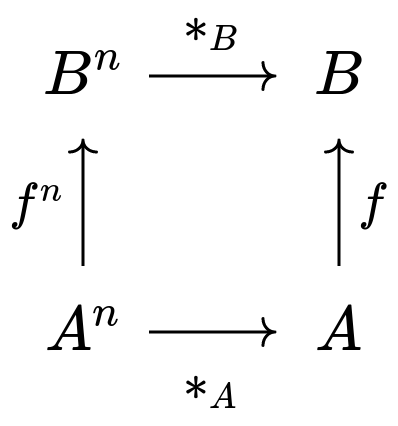
\includegraphics[width=0.25\textwidth]{{./hom.png}}

then the condition that this diagram commutes is equivalent to the expression that $f(a_1*...*a_n) = f(a_1) * ... * f(a_n)$ which is part of the definition of homomorphisms of nary operations.
\end{proof}

We can use this theorem to define the induced $Sets^{\to}$ morphism for a homomorphism of nary operations.

\begin{definition}
let $f: A \to B$ be a homomorphism of nary operations. Then the induced morphism of $d(f)$ is the morphism $(f^n,f)$ in $Sets^{\to}$ from $*_A: A^n \to A$ to $*_B : B^n \to B$
\end{definition}

It follows that the induced $Sets^{\to}$ morphism forms a functor from the category of algebras to $Sets^{\to}$. Every single nary operation corresponds to an object of the topos $Sets^{\to}$. On the other hand, in the more general context of universal algebra, an algebra is defined by a family of nary operations. This necessitates that we define a family of functors to $Sets^{\to}$ for each type of operation on an algebra.

\begin{definition} let $C$ be the category of algebras with signature $(n_1,...n_i)$. Then for any morphism $m: A \to B$ in $C$ there exists an induced $Sets^{\to}$ morphism for each operation in $C$ indexed by $i$ of the form $(f^{n_i}, f)$ from $*_i : A^{n_i} \to A$ to $*_i : B^{n_i} \to B$ yielding an indexed family of functors $F_i : C \to Sets^{\to}$.
\end{definition}

The key property of this representation is that we can use it to reason about algebras of an arbitrary signature by using the topos $Sets^{\to}$. If there is some property that is apparent to some operation of an algebra that can be inferred from its representation in $Sets^{\to}$, then that can probably be generalized from that operation to all other operations in the algebra.

\newpage

Every morphism of algebras induces a morphism in $Sets^{\to}$ of the form $(f^n,f)$. Given such a morphism, we can form its kernel $(ker(f)^n, ker(f))$ in $Sets^{\to}$, which is a functional dataflow relation. These always yield dataflow relations of the form $(C^n, C)$.

\begin{definition}
let $*: A^n \to A$ be a nary operation and let $C$ be a partition of $A$. Then a componentwise dataflow relation is any dataflow relation of the form $(C^n,C)$ associated to the function $*$.
\end{definition}

These componentwise dataflow relations $(C^n, C)$ are precisely the algebraic congruences of any nary operation. Dataflow relations describe how data flows from one place to another. This means that congruences $(C^n,C)$ can be interpreted as saying that the combined $C$ information of all elements in an input tuple determines $C$ information in the output. So algebraic congruences are ways of describing the flow of information from one region to another, which makes them dataflow relations.

\begin{definition}
let $f: A^n \to A$ be a nary operation then we have the following correspondence:

\begin{itemize}
 \item let $C$ be a congruence then the dataflow relation defined by $C$ is the relation $(C^n,C)$.
 \item let $(C^n,C)$ be a componentwise dataflow relation then the algebraic congruence associated with $(C^n, C)$ is the component partition $C$
\end{itemize}
\end{definition}

Then this correspondence between congruences and componentwise dataflow relations leads to a lattice embedding from the lattice of congruences of $A$ represented as an algebra to the lattice of dataflow relations on the $Sets^{\to}$ object $f$, whose image is the set of all componentwise dataflow relations.

\[ i : Con(A) \to Con(f) \]

Although all congruences in algebra are treatable as special types of dataflow relations, the converse is not true. There exist dataflow relations beyond those in classical algebra that are defined componentwise, which can be used to describe other ways that input maps to output by algebraic functions.

For example, let $f: M^2 \to M$ be a magma then we can form a partition $Sym$ on $M^2$ of the form $(a,b) = (b,a)$ that equates two ordered pairs provided that they are equal up to transposition. This is not a componentwise congruence. Nonetheless, by taking partition images, we can still form the dataflow relation $(Sym, f(Sym))$ from it. The partition image equates $x$ and $y$ provided that there exists $a,b$ with $f(ab) = x$ and $f(ba) = y$. Then this dataflow relation describes the bits of information that we can infer from the output from a pair of arguments $x,y$ without knowing the order the arguments are in. This opens up the possibility of considering more types of dataflow relations.

\newpage

In classical algebra and the context of ring theory, there exists an adjunction between ideal lattices associated with any ring map $f: R \to S$. These are defined by the ideal extension and contraction of an ideal under a ring map.

\begin{itemize}
 \item let $f: R \to S$ be a ring map then the extension of $I$ is the ideal closure of $f(I)$
 \item let $f:  R \to S$ be a ring map then the contraction of $I$ is the inverse image $f^{-1}(I)$.
\end{itemize}

Then these define a dual pair of functors $Ideals$ and $Ideals^{-1}$ that define the adjunction between the lattices of ideals of the two rings.

\[ Ideals(F) : Ideals(R) \to Ideals(S) \]
\[ Ideals^{-1}(F) : Ideals(S) \to Ideals(R) \]

These concepts are addressed in the literature under the terms ideal extension and contraction. However, much as with initial and final topologies, we can define these by overloaded images and inverse images. In particular, given an object of the ring map data type and another object of ideal type, then the correct type of mapping can be defined by them by the image and inverse image multimethods.

This integrates the familiar concepts of ideal extension and contraction into our framework of polymorphic images. Having reviewed this concept of ideal extension and contraction, we would like to see if similar concepts arise for algebraic congruences under partition images and inverse images. In fact, as we will see, the situation is much the same.

\begin{itemize}
 \item let $f: A \to B$ be a map of algebras then the congruence image $f(C)$ of a congruence $C$ is the congruence closure of the partition image $f(C)$ in $B$.
 \item let $f: A \to B$ be a map of algebras then the congruence inverse image $f^{-1}(C)$ and the partition inverse image coincide.
\end{itemize}

Then there exists an adjunction between congruence lattices $Con(f) : Con(A) \to Con(B)$ and $Con^{-1}(f) : Con(B) \to Con(A)$ induced by the morphism of algebras $f$. In the special case of rings, there is a mapping $m: Ideals(R) \to Con(R)$ from the ideal lattice of $R$ to its congruence lattice. Then this generalized definition of congruence extension and contraction is a direct generalisation of that concept of extension and contraction from the context of ideals of rings only now applied to congruences. We will now investigate the properties of these congruence images and inverse images using dataflow relations.

\newpage

We will now proceed to examine the preservation and reflection of congruences using the theory of functional dataflow relations. Let $f: A \to B$ be a homomorphism of algebras, and let $C$ be a congruence. Then $(C^n,C)$ is a dataflow relation of $A$ and by the preservation of congruences $(f^n(C^n),f(C))$ is a congruence of $B$.

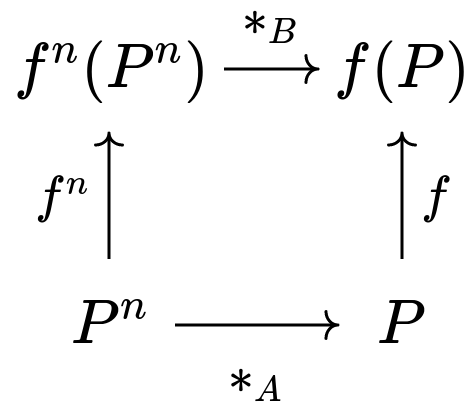
\includegraphics[width=0.24\textwidth]{{./flowpreserve.png}}

The problem with this is the failure of the partition image $f^n(P^n)$ to distribute over products. This leads to the following inequality, which was explained in the section on product functions:

\[ f^n(P^n) \not= (f(P))^n \]

Then this means that for any dataflow relation $(C^n,C)$, its image $(f^n(C^n), f(C))$ is a dataflow relation but it is not a componentwise dataflow relation of any congruence. Instead, it always describes something about how a different collection of information in $f^n(C^n)$ can produce $f(C)$. The failure of the partition image of a congruence to again be a congruence is the reason we have to define the congruence extension.

The image of an ideal under a ring map may always be a subring, but it is not an ideal except under the image extension. By the same token, we apply the congruence extension method to ensure that the partition images of congruences are always again congruences.

The situation for partition inverse images is a different story. Here in fact, we have that partition inverse images preserve congruences of algebras. Given any dataflow relation $(P^n,P)$ then the dataflow inverse image of $(P^n,P)$ is the pair $(f^{-1}(P^n),P)$.

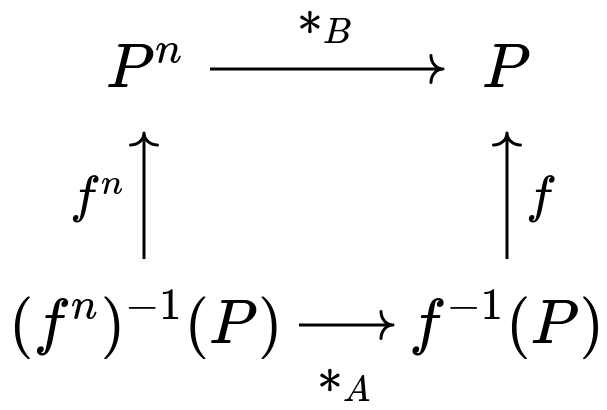
\includegraphics[width=0.28\textwidth]{{./flowreflect.png}}

Then it can be shown that $({(f^n)}^{-1}(P^n),f^{-1}(P))$ can equivalently be expressed as $((f^{-1}(P))^n, f^{-1}(P))$. From this, it implies that partition inverse images reflect algebraic congruences. This leads to our definition of the contraction of congruences.

The two concepts of congruence extension and contraction generalize another concept from the classical algebraic setting of groups, rings, and fields to the setting of universal algebra. At the same time, this demonstrates that this is part of the more general theory of dataflow relations.

\newpage

We will now proceed to determine the inner workings of the contraction of congruences.

\begin{theorem}
let $d: (*_A : A^n \to A) \to (*_B : B^n \to B)$ be a homomorphism of nary operations with components $(f^n,f)$. Then $d$ reflects componentwise dataflow relations.
\end{theorem}

\begin{proof}
let $(C^n,C)$ be a dataflow relation on $*_B : B^n \to B$. Then by theorem 2.5.15 $d$ reflects the congurence $(C^n, C)$ on $*_B : B^n \to B$ back to the congruence $((f^n)^{-1}(C^n), f^{-1}(C))$ is a dataflow relation of $*_A : A^n \to A$. By the fact that product functions distribute over product partitions by inverse images, this is equal to $((f^{-1}(C)^n,f^{-1}(C))$, which is a componentwise dataflow relation.
\end{proof}

The fact that the induced $Sets^{\to}$ morphisms of homomorphisms of nary operations reflect componentwise dataflow relations demonstrates that those homomorphisms themselves reflect congruences.

\begin{corollary}
 let $f: A \to B$ be a homomorphism of algebras then $f$ reflects congruences
\end{corollary}

The reflection of congruences can itself be defined by taking the kernel of the composite map with the projection morphism of the output set along the congruence $C$. There is no similar method for defining the preservation of congruences along algebraic mappings, so congruences are not generally preserved.

As a consequence, congruence extension is defined by taking the congruence closure of the partition image, while congruence contraction and partition inverse images coincide. Then for any category of algebras, we have a dual pair of functors $Con$ and $Con^{-1}$ that can be applied to any morphism $f: A \to B$:

\[ Con(f) : Con(A) \to Con(B) \]
\[ Con^{-1}(f) : Con(B) \to Con(A) \]

The congruence extension $Con(f): Con(A) \to Con(B)$ and the congruence contraction $Con^{-1}(f): Con(B) \to Con(A)$ operators form adjoints of a monotone Galois connection. These congruence extension and contraction operators directly generalize the partition adjunction

In the special case of our polymorphic images implementation, we can define special datatypes for algebras, algebra homomorphisms, and congruences. Then the image of a congruence under a homomorphism will be a congruence determined by congruence extension, and the inverse image will again be a congruence as determined by congruence contraction. In each case, the image and inverse image multimethods will be overloaded based upon data type so that they produce results of the same type.

\newpage

\subsection{Symbolic addresses}
In most computer applications, it is convenient to refer to symbolic addresses rather than referencing partitions directly.

\begin{itemize}
 \item in a list, the parts of the list might be addressed by indices like 0,1,2,3,... and stored using an integer data type.
 \item in a matrix, the parts of the matrix might be addressed by ordered pairs of integers (0,0),(0,1),(1,0),(1,1), representing the data at some position in the matrix.
 \item in a hash table, the memory in the table may be referenced by keys of an arbitrary data type
 \item in a complex number, the real and imaginary parts can be treated as symbolic addresses to information locations of the complex number
 \item in a quaternion, a set of four different keys: h,i,j, and k can be used as symbolic addresses to the information locations of the quaternion
 \item in a conventional computer, an address space is a means of translating symbolic or numeric addresses into data
\end{itemize}

The point of symbolic addresses is that they should represent the canonical units of information located in a data structure. Then composite locations can be constructed from the meet operation of the partition lattice.

\begin{definition}
let $S$ be a structure with $a,b,c$ symbolic addresses to parts of $S$. Then a composite structure containing $\{a,b,c\}$ is defined by the meet of the partitions referenced by the symbols in $\{a,b,c\}$.
\end{definition}

As an example, let $S$ be the class of $3x3$ matrices. Then $\{(0,0),(0,1),(0,2)\}$ refers to the first row in the structure and $\{(0,0),(1,0),(2,0)\}$ refers to the first column. In both cases, the row and column are constructed from the partition meet of the partitions referred to by these symbolic addresses. The information in common between the first column and the first row is the single point $\{(0,0)\}$.

In the case of a conventional computer, sets of memory addresses are combined to form files, processes, and so on. These sets of memory addresses are the partition meet of all the partitions referred to by their components. In any case, regardless of rather you are dealing with a matrix, an address space, a list, or a hash table, composite locations can be formed from smaller ones.

In a concrete computer implementation of symbolic addressing, composite types like the rows and columns of matrices can be represented as sets of symbolic addresses under the hood while still being members of a partition data type. Membership in the partition type ensures that they will have partition images overloaded on them so that symbolic addresses can be mapped back to symbolic addresses.

Symbolic addresses are frequently how we want to interact with and define the places of structures in programs. In turn, these allow us to make more practical use of data flow relations.

\begin{itemize}
 \item let $f(x,y) = (y,x)$ be the function that takes an ordered pair and produces its transposition. Then with respect to symbolic addresses $f : 0 \to 1$ and $f : 1 \to 0$ so that $f$ maps the first index to the second and the second one back to the first.
 \item let $M$ and $N$ be matrices then in the matrix product $MN$ each coordinate $(i,j)$ in the matrix product $MN$ is dependent upon the $ith$ row of $M$ and the $jth$ column of $N$. Then each of these data dependencies form data flow relations on the matrix multiplication operation.
 \item let $u$ and $v$ be vectors then the dot product $u \cdot v$ has that each component $(u \cdot v)_i$ is functionally dependent upon $u_i$ and $v_i$. Each of these functional dependencies form dataflow relations in the topos $Sets^{\to}$.
 \item  let $\mathbb{C}$ be the complex numbers and consider complex conjugation $f(a+bi) = a-bi$. Then the real part maps back to the real part, and the imaginary part maps back to the imaginary part. Both of these conditions form dataflow relations on the complex conjugation of complex numbers.
\end{itemize}

In a conventional computing system, a computation can be specified by a statement like $a \leftarrow b + c$. The assumption is that in any given statement, all memory locations aside from the ones explicitly handled by the computation like $a$ are left alone. It follows that a transformation of memory can be specified only by a set of computations that change given memory locations.

Then in a computation like $a \leftarrow b + c$ we have that $(\{a\},\{b,c\})$ is a dataflow relation describing the movement of $\{b,c\}$ data in to $\{a\}$. The composability of data flow relations is a generalisation of the composition of data dependencies on this level. So if we took $a \leftarrow b+c$ and $d \leftarrow e+f$ and then composed them with $g \leftarrow a+d$. Then $g$ would be dependent upon both the components of $a$ and $d$, so it would be dependent upon $b,c,e$ and $f$ and so on.

It is possible to capture the movement of data between memory addresses using the theory of dataflow relations in $Sets^{\to}$. However, this theory is much more general than that as it allows us to capture the movement of data from any one location to another by a function. This new formulation gives dataflow analysis the highest level of applicability.
\newpage

\chapter{Concluding remarks}
The theory of dataflow relations has been extensively studied [8].  Applications of this theory have been realised in the analysis of parallel programs [9] [10]. In particular, the realisation of the increasing need for the automatic parallelisation of software programs has led to an explosion in need for dataflow analysis and related forms of program analyis.

With this explosion of work in dataflow analysis and program analysis, it is desirable that mathematical foundations should be created for this field of study. These foundations should work on the appropriate level of generality and abstraction so that dataflow analysis has the highest level of applicability.

Previous work on the mathematical foundations of dataflow made us of lattices [8]. We believe that by furthering these models with the use of the topos theory, and in particular the topos $Sets^{\to}$, the field of dataflow analysis can be given firm mathematical foundations.

\section*{References}
[1] Ellerman, D. (2009, February 11). The Logic of Partitions: Introduction to the dual of the logic of subsets. arXiv.Org. https://arxiv.org/abs/0902.1950
\newline \newline
[2]   Kung, J. P. S., Rota, G.-C., Yan, C. H. (2009). Combinatorics: The rota way. Cambridge University Press.
\newline \newline
[3]   Finberg, D., Mainetti, M., Rota, G.-C., Magari, R. (2017). The logic of commuting equivalence relations. In Logic and algebra (pp. 69–96).
\newline \newline
[4] Britz T; Mainetti M; Pezzoli L, 2001, 'Some operations on the family of equivalence relations', in Crapo H; Senato D (ed.), Algebraic Combinatorics and Computer Science. A Tribute To Gian-Carlo Rota, edn. Original, Springer-Verlag Italia, Milan, pp. 445 - 460
\newline \newline
[5] Pudlak, P., Tima, J. (1980). Every finite lattice can be embedded in a finite partition lattice. Algebra Universalis, 10(1), 74–95. https://doi.org/10.1007/bf02482893
\newline \newline
[6] Grätzer, G. (2011). Lattice theory: Foundation. Birkhäuser.
\newline \newline
[7]   McKinsey, J. C. C. (1943). Oystein Ore. Theory of equivalence relations. Duke mathematical journal, vol. 9 (1942), pp. 573–627. Journal of Symbolic Logic, 8(2), 55–56.
\newline \newline
[8] Khedker, U., Sanyal, A, \& Karkare, B. (2017). Data Flow Analysis: Theory and Practice. CRC Press.
\newline \newline
[9] A. J. Bernstein, Analysis of Programs for Parallel Processing, in IEEE Transactions on Electronic Computers, vol. EC-15, no. 5, pp. 757-763, Oct. 1966, doi: 10.1109/PGEC.1966.264565.
\newline \newline
[10] Feautrier P (2001) Array dataflow analysis. In: Pande S, Agrawal D (eds) Compiler optimizations for scalable parallel systems. Lecture notes in computer science, vol 1808, chapter 6. Springer, Berlin, pp 173–216
\newline \newline
[11] Bernier, J (2022) Locus: a computer algebra system based upon topos theory. Available at https://github.com/locusmath/locus
\newline \newline
[12] Goldblatt, R. (2006). Topoi: The categorial analysis of logic. Courier Corporation.
\newline \newline
[14] Johnstone, P. T. (2002). Sketches of an Elephant: A topos theory compendium. Clarendon Press.
\newline \newline
[15] Johnstone, P. T. (2002b). Sketches of an Elephant: A Topos Theory Compendium: Volume 2. Oxford University Press.
\newline \newline
[16] MacLane, S., Moerdijk, I. (1994a). Sheaves in geometry and logic: A first introduction to topos theory. Springer Science; Business Media.



\end{document}
